\documentclass{article}

\usepackage{amsmath, amsthm, amssymb, amsfonts}
\usepackage{thmtools}
\usepackage{graphicx}
\usepackage{setspace}
\usepackage{geometry}
\usepackage{float}
\usepackage{hyperref}
\usepackage[utf8]{inputenc}
\usepackage[english]{babel}
\usepackage{framed}
\usepackage[dvipsnames]{xcolor}
\usepackage{tcolorbox}

%Define the listing package
\usepackage{listings} %code highlighter
\usepackage{color} %use color
\definecolor{mygreen}{rgb}{0,0.6,0}
\definecolor{mygray}{rgb}{0.5,0.5,0.5}
\definecolor{mymauve}{rgb}{0.58,0,0.82}
 
%Customize a bit the look
\lstset{ %
backgroundcolor=\color{white}, % choose the background color; you must add \usepackage{color} or \usepackage{xcolor}
basicstyle=\footnotesize, % the size of the fonts that are used for the code
breakatwhitespace=false, % sets if automatic breaks should only happen at whitespace
breaklines=true, % sets automatic line breaking
captionpos=b, % sets the caption-position to bottom
commentstyle=\color{mygreen}, % comment style
deletekeywords={...}, % if you want to delete keywords from the given language
escapeinside={\%*}{*)}, % if you want to add LaTeX within your code
extendedchars=true, % lets you use non-ASCII characters; for 8-bits encodings only, does not work with UTF-8
frame=single, % adds a frame around the code
keepspaces=true, % keeps spaces in text, useful for keeping indentation of code (possibly needs columns=flexible)
keywordstyle=\color{blue}, % keyword style
% language=Octave, % the language of the code
morekeywords={*,...}, % if you want to add more keywords to the set
numbers=left, % where to put the line-numbers; possible values are (none, left, right)
numbersep=5pt, % how far the line-numbers are from the code
numberstyle=\tiny\color{mygray}, % the style that is used for the line-numbers
rulecolor=\color{black}, % if not set, the frame-color may be changed on line-breaks within not-black text (e.g. comments (green here))
showspaces=false, % show spaces everywhere adding particular underscores; it overrides 'showstringspaces'
showstringspaces=false, % underline spaces within strings only
showtabs=false, % show tabs within strings adding particular underscores
stepnumber=1, % the step between two line-numbers. If it's 1, each line will be numbered
stringstyle=\color{mymauve}, % string literal style
tabsize=2, % sets default tabsize to 2 spaces
title=\lstname % show the filename of files included with \lstinputlisting; also try caption instead of title
}
%END of listing package%
 
\definecolor{darkgray}{rgb}{.4,.4,.4}
\definecolor{purple}{rgb}{0.65, 0.12, 0.82}
 
%define Javascript language
\lstdefinelanguage{JavaScript}{
keywords={typeof, new, true, false, catch, function, return, null, catch, switch, var, if, in, while, do, else, case, break, let, fun, and, with, match, then, type, of, ref, mutable, for, to, done, exception, raise, failwith},
keywordstyle=\color{blue}\bfseries,
ndkeywords={class, export, boolean, throw, implements, import, this},
ndkeywordstyle=\color{darkgray}\bfseries,
identifierstyle=\color{black},
sensitive=false,
comment=[l]{//},
morecomment=[s]{/*}{*/},
commentstyle=\color{purple}\ttfamily,
stringstyle=\color{red}\ttfamily,
morestring=[b]',
morestring=[b]"
}
 
\lstset{
language=JavaScript,
extendedchars=true,
basicstyle=\footnotesize\ttfamily,
showstringspaces=false,
showspaces=false,
numbers=left,
numberstyle=\footnotesize,
numbersep=9pt,
tabsize=2,
breaklines=true,
showtabs=false,
captionpos=b
}

\colorlet{LightGray}{White!90!Periwinkle}
\colorlet{LightOrange}{Orange!15}
\colorlet{LightGreen}{Green!15}

\newcommand{\HRule}[1]{\rule{\linewidth}{#1}}

\NewEnviron{NORMAL}{% 
    \scalebox{2}{$\BODY$} 
} 

\declaretheoremstyle[name=Theorem,]{thmsty}
\declaretheorem[style=thmsty,numberwithin=section]{theorem}
\tcolorboxenvironment{theorem}{colback=LightGray}

\declaretheoremstyle[name=Proposition,]{prosty}
\declaretheorem[style=prosty,numberlike=theorem]{proposition}
\tcolorboxenvironment{proposition}{colback=LightOrange}

\declaretheoremstyle[name=Principle,]{prcpsty}
\declaretheorem[style=prcpsty,numberlike=theorem]{principle}
\tcolorboxenvironment{principle}{colback=LightGreen}

\setstretch{1.2}
\geometry{
    textheight=9in,
    textwidth=5.5in,
    top=1in,
    headheight=12pt,
    headsep=25pt,
    footskip=30pt
}

% ------------------------------------------------------------------------------

\begin{document}

% ------------------------------------------------------------------------------
% Cover Page and ToC
% ------------------------------------------------------------------------------

\title{ \normalsize \textsc{}
		\\ [2.0cm]
		\HRule{1.5pt} \\
		\LARGE \textbf{\uppercase{Paradigmi di Programmazione}
		\HRule{2.0pt} \\ [0.6cm] \LARGE{Corso A} \vspace*{10\baselineskip}}
		}
\date{}
\author{\textbf{Autore} \\ 
		Giuseppe Acocella \\
		2024/25\\}

\maketitle
\newpage

\tableofcontents

\newpage

%\begin{figure}[htbp]
    %\center
    %\includegraphics[scale=0.4]{img/classiComplessita2.png}
%\end{figure}

\newpage

\section{OCaml}

Descriviamo le caratteristiche dell'OCaml e forniamo snippet di codice relativi all'argomento trattato.

\subsection{Dichiarazioni e tipi variabili}

\paragraph{Variabili:} Le variabili, una volta creato il binding ed assegnato un valore non è possibile modificarle.

\paragraph{Dichiarazione:} La dichiarazione di una variabile avviene con la parola chiave \textbf{let} e può essere utilizzata per dichiarare ogni tipo di variabile, anche di tipo \textbf{funzione}.

\paragraph{Espressioni:} Ogni riga di codice è un espressione, e mai un comando. Dunque essendo che stiamo aderendo al paradigma funzionale, non ci è permesso apportare modifiche ad \textbf{ambiente} e \textbf{memoria}.
Le \textbf{espressioni} possono quindi contenere \textbf{bindings}.

\vspace*{10px}

\begin{lstlisting}[language=JavaScript]
    let x = 5;;
\end{lstlisting}

\vspace*{-15px}

\subsubsection{Tipi, Cast ed Overload}

\paragraph{Tipi:} Enumeriamo i tipi base disponibili:
\begin{enumerate}
    \item \textbf{int}: numeri interi
    \item \textbf{float}: numeri frazionari *floating point* a doppia precisione
    \begin{enumerate}
        \item \textbf{Operatori}: $+. \:\:\: -. \:\:\: *. \:\:\: /. $
    \end{enumerate}
    \item \textbf{bool}: valori di verità (booleani): `true` o `false`
    \begin{enumerate}
        \item \textbf{Operatori}: $  \& \& \:\:\: || \:\:\: not $
    \end{enumerate}
    \item \textbf{char}: singoli caratteri (racchiusi tra apici: `'a'` )
    \item \textbf{string}: stringhe (racchiuse tra virgolette: `"abcd"` )
    \begin{enumerate}
        \item \textbf{Concatenazione}: $str_{1}\:\wedge\:str_{2}$
        \item \textbf{Overload}: Notiamo quindi che non verrà castato automaticamente un $int$ a $float$, infatti esistono le operazioni specifiche per i float.
    \end{enumerate}
    \item \textbf{unit}: tipo usato in casi particolari (simile a `void` in altri linguaggi), prevede come unico valore `()`
\end{enumerate}

\paragraph{Cast:}
In \textbf{OCaml} ogni tipo di cast è \textbf{esplicito}, dato che il sistema di tipi è molto \textbf{rigido}. Questo ci permette di poter sfruttare anche il \textbf{type inference} dell' \textbf{OCaml}, dato che nulla viene lasciato al caso.
\vspace*{10px}
\begin{lstlisting}[language = JavaScript]
    let c = 'a' ;;
    int_of_char c ;;
\end{lstlisting}
\vspace*{-10px}

Questi tipi di cast esistono quindi da ogni e verso ogni tipo base.

\newpage

\subsection{Tuple e Liste}

Mostriamo questi due tipi "composti", ognuno caratterizzato da specifiche particolari:

\begin{enumerate}
    \item \textbf{Tuple}: Sono strutture non omogenee, definite anche n-uple, che variano in lunghezza, possono quindi contenere elementi di tipo diverso
    \vspace*{10px}
    \begin{lstlisting}[language = JavaScript]
    let t = (10,"hello",12.5);;
    \end{lstlisting}
    \vspace*{-10px}
    \item \textbf{Liste}: Strutture omogenee, su cui è possibile effettuare varie operazioni di natura induttiva grazie alla ricorsione. Si mostrano queste operazioni nei capitoli successivi dedicati al \textbf{Pattern Matching}.
    \vspace*{10px}
    \begin{lstlisting}[language = JavaScript]
    let numeri = [3; 5; -1; 9; 14; 21] ;;
    \end{lstlisting}
    \vspace*{-10px}
\end{enumerate}

\subsection{Funzioni}

Le \textbf{funzioni} sono il nucleo del paradigma funzionale. Ricordiamo che sono \textbf{espressioni} come tutte le altre e dunque possono essere legate ad un identificatore grazie ad un binding.

\begin{enumerate}
    \item \textbf{Funzione Anonima}: Mostriamo una funzione nella sua essenza, prima ancora di effettuare il binding.
    \vspace*{10px}
    \begin{lstlisting}[language = JavaScript]
    fun x -> x + 1 ;;
    \end{lstlisting}
    \vspace*{-10px}
    \item \textbf{Invocazione di Funzione}: Proprio come nel lambda calcolo possiamo invocare una funzione simile.
    \vspace*{10px}
    \begin{lstlisting}[language = JavaScript]
    (fun x -> x + 1) 3;;
    \end{lstlisting}
    \begin{figure}[htbp]
    \center
    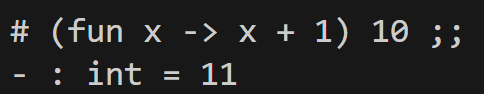
\includegraphics[scale=0.35]{img/invocazioneFunzione.png}
    \end{figure}
    \vspace*{-10px}
\end{enumerate}

\vspace{15px}

Dunque notiamo che questo tipo di notazione è fortemente influenzato dallo stile del \textbf{Lambda Calcolo}.

\newpage

\subsubsection{Currying e Zucchero Sintattico}

Seguendo lo stile del \textbf{Lambda Calcolo} non è possibile avere più di un parametro in binding in una funzione. Questo stile è detto \textbf{Curryed}. Mostriamo quindi tutte le possibili rappresentazioni che l'\textbf{OCaml} offre:

\begin{enumerate}
    \item \textbf{Stile Curryed}:
    \vspace*{10px}
    \begin{lstlisting}[language = JavaScript]
    fun x -> fun y -> x+y ;;
    \end{lstlisting}
    \vspace*{-10px}
    \item \textbf{Stile Semplificato}:
    \vspace*{10px}
    \begin{lstlisting}[language = JavaScript]
    fun x y -> x+y ;;
    \end{lstlisting}
    \vspace*{-10px}
\end{enumerate}

\begin{figure}[htbp]
    \center
    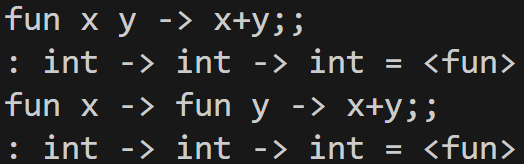
\includegraphics[scale=0.4]{img/notazioneFunzioni.png}
    \caption{Notiamo che le due funzioni si equivalgono in entrambe le notazioni dato che hanno anche lo stesso tipo}
\end{figure}

\vspace*{15px}

\subsubsection{Binding Funzione ad Identificatore}

Il modo più comune per definire funzioni è quello di legarle ad un identificatore. Mostriamo due diversi modi di effettuare questo \textbf{binding}.

\begin{enumerate}
    \item \textbf{Versione base}: Versione basata sulla notazione $->$
    \vspace*{10px}
    \begin{lstlisting}[language = JavaScript]
    let somma = fun x y -> x+y ;;
    somma 3 4 ;;
    \end{lstlisting}
    \vspace*{-10px}
    \item \textbf{Versione semplificata}: Versione basata sullo zucchero sintattico offerto dall'OCaml, questo stile è detto Curryed.
    \vspace*{10px}
    \begin{lstlisting}[language = JavaScript]
    let somma x y = x+y ;;
    somma 3 4;;
    \end{lstlisting}
    \vspace*{-10px}
    
\end{enumerate}

\newpage

\subsubsection{Notazione Curryed vs Tupla Parametri}

Abbiamo già definito quale sia il modo più comune per definire funzioni, ossia lo stile \textbf{Curryed}. Ma nulla vieta l'utilizzo di una tupla per il passaggio dei parametri. Ci sono però delle differenze:

\begin{enumerate}
    \item \textbf{Notazione Curryed Parametri}: 
    \vspace*{10px}
    \begin{lstlisting}[language = JavaScript]
    let somma x y = x+y ;;
    somma 3 4;;
    \end{lstlisting}
    \vspace*{-15px}
    Questa \textbf{permette} l'\textbf{applicazione parziale} di funzione, dato che nulla vieta il passaggio di un parametro singolo.

    \item \textbf{Notazione Tupla Parametri}: 
    \vspace*{10px}
    \begin{lstlisting}[language = JavaScript]
    let somma (x, y) = x+y ;;
    somma (3, 4);;
    \end{lstlisting}
    \vspace*{-15px}
    Questa \textbf{vieta} l'\textbf{applicazione parziale} di funzione, dato che l'applicazione di funzione necessita un parametro che sia una tupla.
    
\end{enumerate}

\vspace*{20px}

\subsubsection{Funzioni Ausiliarie}

Una funzione può anche essere visibile solo nello scope di una specifica \textbf{espressione} che la necessita. Mostriamo e descriviamo un esempio.

\vspace*{10px}
    \begin{lstlisting}[language = JavaScript]
    let sol a b c =
    let delta =
        b*.b -. 4.*.a*.c
    in
        ( (-.b +. sqrt delta) /. (2.*.a) , (-.b -. sqrt delta) /. (2.*.a) ) ;; 
    \end{lstlisting}
\vspace*{-10px}

\begin{enumerate}
    \item \textbf{sol}: Funzione esterna che richiede tre parametri $a,\: b,\: c$.
    \item \textbf{delta}: Funzione ausiliaria visibile solo nell'espressione a \textit{riga 5}, che non prende argomenti, dato che utilizza come dati quelli contenuti nei \textit{parametri formali} della funzione \textit{sol}.
    \item \textbf{Espressione eseguita}: Alla fine, si esegue il calcolo dell'espressione a \textit{riga 5} che si basa su funzione ausiliare e su parametri della funzione esterna.
\end{enumerate}

\newpage

\subsection{Controllo Flusso e Iterazione}

Abbiamo la necessità di stabilire gli \textit{if} per il controllo del flusso
e successivamente anche come reiterare in questo linguaggio determinate espressioni.

Ricordiamo però che essendo questo linguaggio puramente funzionale (per ora), non ci è permesso modificare \textbf{ambiente} e \textbf{memoria}. Dunque non effettueremo iterazioni proprie ma invocheremo le funzioni ricorsivamente.

\begin{enumerate}
    \item \textbf{if}: Mostriamo il controllo del flusso base.
    \vspace*{10px}
    \begin{lstlisting}[language = JavaScript]
    let x = 23 ;;
    let y = if x>10 then 1 else 0 ;;  
    \end{lstlisting}
    \vspace*{-10px}

    \item \textbf{Ricorsione Base}: Mostriamo esempio sul Fibonacci.
    \vspace*{10px}
    \begin{lstlisting}[language = JavaScript]
    let rec fibonacci n =
    if n=0 || n=1 then n
    else fibonacci (n-1) + fibonacci (n-2);;
    \end{lstlisting}
    \vspace*{-10px}
    Notiamo che in questo caso è necessario definire \textit{fibonacci} come funzione ricorsiva \textit{let rec}. Questo è zucchero sintattico che permette al compilatore di sapere che avrà bisogno di utilizzare una sorta di \textbf{combinatore Y} come abbiamo visto per il $\lambda \: - \: $ calcolo.
\end{enumerate}

\vspace*{20px}

\subsubsection{Funzioni Mutuamente Ricorsive}
Mostriamo un semplice esempio di funzioni mutuamente ricorsive utilizzando il costrutto \textbf{match} che si approfondirà durante il \textbf{pattern matching}.

\vspace*{10px}
\begin{lstlisting}[language = JavaScript]
    let rec pari n =
    match n with
    | 0 -> true
    | x -> dispari (x-1)
    
    and dispari n =
    match n with
    | 0 -> false
    | x -> pari (x-1) ;;
\end{lstlisting}
\vspace*{-10px}

\newpage

\subsection{Type Inference}

Tutta la rigidità imposta sui tipi di permette di poter sfruttare un potentissimo \textbf{type inference}. Questo perchè \textbf{staticamente} il compilatore riesce a derivare quali siano i tipi dei parametri passati e il tipo della funzione stessa grazie a tutti i vincoli imposti precedentemente.

\vspace*{10px}
\begin{lstlisting}[language = JavaScript]
    let sum_if_true test first second =
    (if test first then first else 0)
    + (if test second then second else 0);;
\end{lstlisting}

\vspace*{-20px}

\begin{figure}[htbp]
    \center
    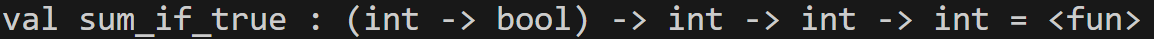
\includegraphics[scale=0.4]{img/typeInference1.png}
\end{figure}

In questo caso ad esempio notiamo che il compilatore riesce perfettamente a capire di che tipo siano tutti i parametri e la funzione stessa prima ancora di valutarla definendoli. Questo per i seguenti motivi:

\begin{enumerate}
    \item \textit{test}: deve ritornare un booleano, dato che \textit{if (test)}.
    \item \textit{first} e \textit{second}: devono avere lo stesso tipo di $0$ (quindi \textbf{int}) dato che non importa quale ramo dell'if si scelga a runtime, questi devono certamente arrivare allo stesso tipo.
    \item \textit{test}: se quindi \textit{test} prendeva in input o \textit{first} o \textit{second} allora sappiamo inferire anche sul suo tipo in ingresso. Dunque il suo tipo complessivo dovrà essere:
    \[ (\: int \: -> \: bool \:) \]
\end{enumerate}

\vspace*{20px}

\subsubsection{Polimorfismo} A volte delle funzioni necessitano un tipo generico per stabilire cosa ritorneranno o cosa prenderanno come parametro. Un esempio è la funzione identità che prende un elemento di qualsiasi tipo e ritorna l'elemento stesso, il cui tipo corrisponde esattamente al tipo in partenza. Concetto simile al tipo \textbf{generics} in TypeScript.

\begin{figure}[htbp]
    \center
    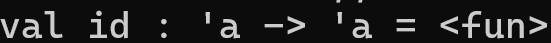
\includegraphics[scale=0.4]{img/polimorfismo.png}
    \caption{a' indica il tipo generico}
\end{figure}

\newpage

\subsection{Pattern Matching}

Il Pattern Matching dell'OCaml è un operazione molto potente che permette di categorizzare tutte le tipologie dato un determinato dato in ingresso. Ha molti elementi in comune con un classico \textbf{switch} ma più ampio. Spesso infatti il \textbf{Pattern Matching} lo si utilizza sulla struttura di un dato complesso come liste e tuple.

Mostriamo un esempio su ricorsione, uno su destrutturazione di liste e uno sulla gestione delle tuple:

\begin{enumerate}

\item \textbf{Fibonacci Ricorsivo}:

\vspace*{10px}
\begin{lstlisting}[language = JavaScript]
let rec fibonacci n =
    match n with
    | 0 -> 0
    | 1 -> 1
    | _ -> fibonacci (n-1) + fibonacci (n-2);;
\end{lstlisting}

\vspace*{-20px}

\item \textbf{Lunghezza lista}:

\vspace*{10px}
\begin{lstlisting}[language = JavaScript]
let rec lenList lst =
    match lst with
    | [] -> 0
    | a::lst1 -> 1 + lenList lst1;;
\end{lstlisting}

\vspace*{-20px}

\item \textbf{Primo true nella tupla}:

\vspace*{10px}
\begin{lstlisting}[language = JavaScript]
let first_true t =
    match t with
    | (true,_,_) -> 1
    | (false,true,_) -> 2
    | (false,false,true) -> 3
    | (false,false,false) -> -1;;
\end{lstlisting}

\vspace*{-20px}

\end{enumerate}

\paragraph{Operazioni strutturali su liste}

Grazie al \textbf{Pattern Matching} riusciamo ad effettuare molte operazioni ricorsive basate sulla destrutturazione di liste. Ricordiamo però che le liste in OCaml sono realizzate come \textbf{Singly Linked List}, dunque manteniamo un riferimento alla testa della lista e passiamo ai successivi. Questo vuol dire che per concatenare due liste è necessario creare un nuovo puntatore, dato che se aggiungessimo semplicemente "in coda" alle liste già esistenti staremmo modificando la lista di partenza.

\vspace*{10px}

\paragraph{Esaustività}

Dato che l'OCaml non assume nulla, è necessario coprire la casistica per ogni possibile valore della variabile data in input al match. Questo non è obbligatorio ma se viene costruito un \textbf{Pattern Matching} non esaustivo viene sollevato un warning.

\newpage

\subsection{Funzioni Higher Order}

Abbiamo mostrato come sia possibile effettuare ricorsione strutturale su liste con il \textbf{Pattern Matching}. Spesso però eseguiremo operazioni molto simili in funzioni diverse. Infatti molte volte ci troveremo ad esempio a "scorrere tutti gli elementi" oppure "applicare una funzione a tutti", o ancora "filtrare in base a $ predicato_{x} $". Possiamo quindi stabilire delle funzioni che acquisiscono funzioni/predicati e liste su cui vogliamo che operino. In questo modo avremo una disponibilità di "operazioni macro" a cui fare riferimento. Elenchiamone alcune:

\begin{enumerate}
\item \textbf{Map}:
\vspace*{10px}
\begin{lstlisting}[language = JavaScript]
let rec map f lis =
    match lis with
    | [] -> []
    | x::lis1 -> f x::map f lis1 ;;
\end{lstlisting}

\vspace*{-20px}

\item \textbf{Filter}:
\vspace*{10px}
\begin{lstlisting}[language = JavaScript]
let rec filter p lis =
    match lis with
    | [] -> []
    | x::lis1 -> if p x then x::filter p lis1
                 else filter p lis1 ;;
\end{lstlisting}

\vspace*{-20px}

\item \textbf{For All}:
\vspace*{10px}
\begin{lstlisting}[language = JavaScript]
let rec forall p lis =
    match lis with
    | [] -> true
    | x::lis1 -> if p x then forall p lis1
                 else false ;;
\end{lstlisting}

\vspace*{-20px}

\item \textbf{Fold (from) Right}:
\vspace*{10px}
\begin{lstlisting}[language = JavaScript]
let rec fold_right f lis a =
    match lis with
    | [] -> a
    | x::lis1 -> f x (fold_right f lis1 a) ;;
\end{lstlisting}

\vspace*{-20px}
\end{enumerate}

\paragraph{Esempio di Applicazione} Mostriamo un esempio di applicazione di somma di tutti gli elementi di una lista con l'utilizzo della \textbf{Fold Right}.

\vspace*{10px}
\begin{lstlisting}[language = JavaScript]
    let somma lis = fold_right (+) lis 0 ;;
    somma [3;2;4] ;;
\end{lstlisting}

\vspace*{-20px}

\newpage

\subsection{Tipi Custom}

Rappresentiamo come definire nuovi tipi custom.

\subsubsection{Record e Definizione Type}

Una delle operazioni principali sui tipi è quella di stabilirne uno nuovo:

\vspace*{10px}
\begin{lstlisting}[language = JavaScript]
    type data = int*int*int ;;
\end{lstlisting}

\vspace*{-20px}

In questo modo stiamo quindi definendo un nuovo tipo come tupla, sapendo che le tuple si basano sul prodotto cartesiano di insiemi.

\vspace*{15px}

\paragraph{Record} Questo tipo non è nient'altro che una maniera più avanzata di utilizzo del prodotto cartesiano di insiemi.

\vspace*{10px}
\begin{lstlisting}[language = JavaScript]
    type punto_2d = { x: float; y: float; } ;;
    let p = { x = 3.; y = -4. } ;;
\end{lstlisting}

\vspace*{-20px}

Elenchiamo un po' di caratteristiche di questa definizione di tipo:

\begin{enumerate}
    \item I Record sono \textbf{immutabili}, dunque sono rappresentati come oggetti ma non equivalgono a questi ultimi.
    \vspace*{15px}
    \item Non esiste nessun metodo, possiamo si assegnare delle funzioni ai campi del record, ma queste ultime non vedranno gli altri campi del record in questione dato che non esiste nessun costrutto simile al \textbf{this}.
    \vspace*{15px}
    \item La \textbf{dot notation} permette un accesso diretto ai campi, quindi un record non ha la necessità di mantenere la "posizionalità" dei campi.
    \vspace*{15px}
    \item il \textbf{functional updating} non è nient'altro che la creazione di un nuovo record partendo da uno già esistente e modificando alcuni dei suoi campi.
    \vspace*{10px}
\begin{lstlisting}[language = JavaScript]
    type persona = {nome: string; cognome: string; via: string; citta: string} ;;
    
    let padre = {nome:"Mario" ; cognome:"Rossi" ; via:"Via Bianchi" ; citta:"Roma"} ;;
    let figlia = { padre with nome = "Bianca" } ;;
\end{lstlisting}

\vspace*{-20px}
\end{enumerate}

\newpage

\subsubsection{Tipi Unione/Somma - Variant}

Grazie ai tipi \textbf{variant} è possibile generare un nuovo \textbf{tipo} come \textbf{unione} di tipo già esistenti. 
\begin{enumerate}
\item \textbf{TypeScript}: 
\vspace*{10px}
\begin{lstlisting}[language = JavaScript]
    type t = string | int
\end{lstlisting}
\vspace*{-20px}

\item \textbf{OCaml}: 
\vspace*{10px}
\begin{lstlisting}[language = JavaScript]
    type numero_testo =
        | Txt of string
        | Num of int ;;
\end{lstlisting}
\vspace*{-20px}
\end{enumerate}

Notiamo delle differenze, infatti l'\textbf{OCaml} richiede un \textbf{etichetta} detta anche \textbf{costruttore}, che segnali di quale "partizione" faccia parte nel nuovo tipo unione definito.

\paragraph{Tipi Strutturali Ricorsivi} Possiamo quindi definire le \textbf{liste} come caso particolare di tipo \textbf{union ricorsivo}.

\vspace*{10px}
\begin{lstlisting}[language = JavaScript]
    type lista_di_int =
        | Nil
        | Elem of int * lista_di_int ;;
    
    let lst = Elem (3 ,Elem (4, Elem (6,Nil))) ;;
\end{lstlisting}
\vspace*{-20px}

\subsubsection{Tipi Enumerazione}

Anche in \textbf{OCaml} è possibile definire le \textbf{enum}, utilizzando solo \textbf{costruttori} è possibile infatti raggiungere lo stesso significato di una normale \textbf{enum}.

\vspace*{10px}
\begin{lstlisting}[language = JavaScript]
    type giorno = Lun | Mar | Mer | Gio | Ven | Sab | Dom ;;
\end{lstlisting}
\vspace*{-20px}

Questo ci permette quindi di eseguire controlli sul tipo grazie al \textbf{Pattern Matching}:

\vspace*{10px}
\begin{lstlisting}[language = JavaScript]
    let is_weekend g =
        match g with
        | Sab | Dom -> true
        | _ -> false ;;
\end{lstlisting}
\vspace*{-20px}

\subsubsection{Tipi Opzione}

I tipi \textbf{opzione} sono particolari tipi \textbf{variant} che consentono di stabilire se esiste o meno un dato grazie ai costruttori \textit{Some} e \textit{None}. In questo modo possiamo gestire il ritorno di nessun valore. 

\vspace*{10px}
\begin{lstlisting}[language = JavaScript]
    type A option =
        | Some of A
        | None ;;
\end{lstlisting}
\vspace*{-20px}

\newpage

\subsection{Cenni Programmazione Imperativa}

In OCaml è anche possibile scrivere codice secondo il paradigma imperativo, abbiamo però bisogno di nuovi tipi di dati che ci permettano di aggiornare e variare il loro contenuto. 
Ricordiamo però che l'utilizzo del paradigma imperativo richiede delle regole di "buon uso" che permettono di non "distruggere" tutta la rigidità costruita fino ad ora grazie al paradigma funzionale. Elenchiamo alcune buone norme:
\begin{enumerate}
    \item Si preferisce l'utilizzo del funzionale all'imperativo.
    \item Ogni funzione imperativa, se scritta, deve essere incapsulata per fare in modo che il suo stato non influenzi le funzioni "indipendenti" definite nel resto del codice.
\end{enumerate}

\subsubsection{Tipi di dato}

\vspace*{10px}

Elenchiamo i tipi di dati:

\vspace*{10px}

\begin{enumerate}
    \item \textbf{Variabili (Riferimenti)}: Abbiamo la necessità di stabilire nuove variabili che siano modificabili. Mostriamone la sintassi:

\begin{enumerate}
\item \textbf{Dichiarazione}:
    \vspace*{10px}
\begin{lstlisting}[language = JavaScript]
    let x = ref 12 ;;
\end{lstlisting}

\begin{figure}[htbp]
    \center
    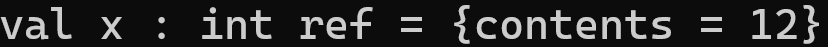
\includegraphics[scale=0.35]{img/ref1.png}
\end{figure}

\vspace*{-5px}
\item \textbf{Accesso a Contents}:
\vspace*{10px}
\begin{lstlisting}[language = JavaScript]
    x.contents ;;
    x.contents <- 13;;
\end{lstlisting}
\vspace*{-20px}
\item \textbf{Sintassi propria di Accesso e Assegnamento}:
\vspace*{10px}
\begin{lstlisting}[language = JavaScript]
    !x ;;
    x := 14 ;;
\end{lstlisting}
\vspace*{-20px}
\end{enumerate}

Ricordiamo che l'accesso a \textbf{Contents} del punto $b$ e le operazioni di \textbf{Accesso} e \textbf{Assegnamento} sono identiche.

\vspace*{15px}

\item \textbf{Array}: Gli array sono modificabili, a differenza delle liste fino ad ora osservate. Mostriamo la loro sintassi:

\begin{lstlisting}[language = JavaScript]
    let a = [|3;5;2|] ;;
    let n = Array.length a;;
    let e = a.(1) ;;
    a.(1) <- 6 ;; 
\end{lstlisting}
\vspace*{-20px}

In ordine abbiamo rappresentato \textbf{dichiarazione e inizializzazione}, \textbf{utilizzo di metodo}, \textbf{accesso a campo} e \textbf{assegnamento a campo}.

\newpage

\item \textbf{Record Mutabili}: Possiamo definire dei tipi \textbf{record} e successivamente stabilire quali campi vogliamo che siano \textbf{variabili}:

\begin{lstlisting}[language = JavaScript]
    type persona = 
    {
        nome: string;
        cognome: string;
        mutable eta: int;
    }
\end{lstlisting}
\vspace*{-20px}

\item \textbf{Eccezioni}: Possiamo gestire gli errori come negli altri linguaggi, \textbf{OCaml} offre quindi la possibilità di sollevare eccezioni, proprio come il \textit{throw} in JS. Mostriamo degli esempi:

\begin{lstlisting}[language = JavaScript]
    exception Lista_vuota ;;
    exception Stringa_errata of string ;;
    raise Lista_vuota;;
    failwith "messaggio di errore" ;;
\end{lstlisting}
\vspace*{-20px}
    
\end{enumerate}

\subsubsection{Comandi Iterativi}

Dato che abbiamo mostrato come sia possibile aggiornare un valore di una variabile, ora possiamo iterare aggiornando degli indici, non essendo più costretti ad effettuare ricorsione.

\begin{enumerate}
    \item \textbf{While}:
\begin{lstlisting}[language = JavaScript]
    let x=ref 10 in
    while !x>0 do
        print_endline (string_of_int !x) ;
        x := !x/2
    done
\end{lstlisting}
\vspace*{-20px}

    \item \textbf{For}:
\begin{lstlisting}[language = JavaScript]
    for i = 1 to 10 do
        print_endline (string_of_int i)
    done ;;
\end{lstlisting}
\vspace*{-20px}

\end{enumerate}

\newpage

\section{Macchine Astratte e Interpreti}

Tutte le macchine attuali si ispirano ad un antico modello, detto \textbf{modello di Von Neumann}. Questo prevedeva l'interazione tra due elementi principali, ossia:
\begin{enumerate}
    \item \textbf{Unità centrale di elaborazione}
    \item \textbf{Memoria}
\end{enumerate}

Grazie a questo schema le macchine di oggi riescono ad eseguire tutte le operazioni che gli assegniamo.

Questa esecuzione di operazioni avviene a sua volta secondo uno schema preciso:

\paragraph{Ciclo Fetch, Decode, Execute} Grazie a questo ciclo, le istruzioni vengono prima caricate dalla memoria \textbf{Fase Fetch}, successivamente vengono tradotte da linguaggio macchina in binario \textbf{Fase Decode} e successivamente vengono eseguite \textbf{Fase Execute}.

\subsection{Tipi di linguaggi} Un linguaggio dunque per essere elaborato da una macchina deve essere convertito in linguaggio macchina. Esistono 3 tipi di approccio:

\begin{enumerate}
    \item \textbf{Compilato}: Viene compilato tutto il sorgente e vengono eseguiti dei controlli a tempo statico. Dunque tutto il sorgente viene compilato e reso eseguibile.
    \item \textbf{Interpretato}: L'interpretazione esegue "riga per riga" i comandi del sorgente. In questo caso non è quindi possibile eseguire dei controlli a tempo statico.
    \item \textbf{Misto}: Questa metodologia utilizza un compilatore intermedio che compila il \textbf{source} in \textbf{bytecode}. Successivamente viene dato il \textbf{bytecode} ad un interprete che lo esegue riga per riga.
\end{enumerate}

\subsection{Macchina Astratta}

Una Macchina Astratta esegue comandi step by step, omettendo i dettagli più a basso livello.

\vspace*{15px}

\begin{figure}[htbp]
    \center
    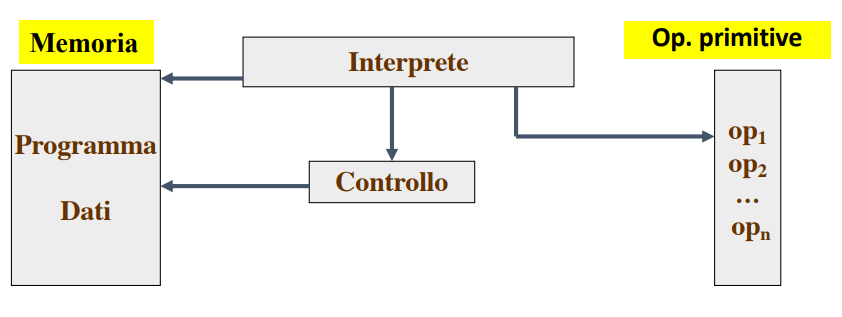
\includegraphics[scale=0.55]{img/macchinaAstratta1.png}
\end{figure}

\newpage

\subsubsection{Macchina Astratta e Linguaggi}

Elenchiamo tutti gli elementi necessari alla realizzazione di una macchina astratta di un linguaggio su una macchina host:

\begin{enumerate}
    \item $\textbf{L}$: Linguaggio ad alto livello
    \item $\textbf{M}_{L}$: Macchina astratta del linguaggio L
    \item $\textbf{M}_{H}$: Macchina fisica host (ospite) 
\end{enumerate}

Questi elementi interagiscono tra di loro in modo diverso in base a che tipo di traduzione scegliamo tra linguaggio ad alto livello \textbf{$L$} e macchina fisica \textbf{$M_{H}$}. 

\begin{enumerate}
    \item \textbf{Interprete Puro}: La macchina astratta \textbf{$M_{L}$} permette la traduzione riga per riga del linguaggio \textbf{$L$} per essere eseguito dalla macchina host \textbf{$M_{H}$}.
    \item \textbf{Compilatore Puro}: Non esiste una vera e propria macchina astratta \textbf{$M_{L}$}, infatti viene direttamente tradotto tutto il sorgente \textbf{$L$} in linguaggio macchina di \textbf{$M_{H}$}.
    \item \textbf{Misto}: Questo tipo di approccio si appoggia su una prima fase di compilazione da sorgente \textbf{$L$} in linguaggio di una macchina astratta intermedia \textbf{$M_{L}$} che interpreterà passo passo il compilato in "bytecode".
\end{enumerate}

\subsubsection{RTS - Run Time Support}

Durante il \textbf{tempo di esecuzione} è necessario fornire supporto al programma che avrà bisogno di un contesto per poter runnare in maniera solida. Il ruolo dell'\textbf{RTS} quindi è quello di fornire supporto al programma main. Nel linguaggio C ad esempio si occupa della chiusura/apertura dei record di attivazione e anche della gestione dello stack e dell'heap.

\subsubsection{Fasi Front/Back End}

Elenchiamo delle macrofasi della compilazione/interpretazione:

\begin{enumerate}
    \item \textbf{Front End}: Il front end della compilazione si occupa di tutti gli aspetti del linguaggio ad alto livello, quindi il suo scanning, parsing e gestione semantica.
    \begin{enumerate}
        \item \textbf{Scanning}: Si acquisisce tutto il sorgente e lo si scannerizza per definirne tutti i token. Questo dunque produrrà una lista di tanti token diversi.
        \item \textbf{Parsing}: Data la lista di token, si verifica in questa fase se sia o meno possibile formare quella sequenza di token data una specifica grammatica del linguaggio in questione. Si produce quindi un \textbf{AST}, ossia un Abstract Syntax Tree.
        \item \textbf{Semantica}: Dato un \textbf{AST} possiamo quindi stabilire il suo significato. Elenchiamo le possibili sottofasi:
        \begin{enumerate}
            \item \textbf{Type Checking}: Questo controllo viene eseguito staticamente nei linguaggi compilati. Questo permette di escludere tutti gli errori causati da interazioni tra tipi non compatibili. Nei linguaggi interpretati come JS, non viene effettuata un analisi statica di tipi, infatti ogni variabile si porta dietro un \textbf{descrittore} che contiene tutte le sue caratteristiche di tipo.

            \newpage
            
            Dunque durante l'esecuzione, il confronto tra descrittori permette di segnalare potenziali errori di tipo. Questo approccio non è per nulla efficiente e rigido, dato che dipendera quasi esclusivamente dall'andamento del programma.

            \item \textbf{Ottimizzazioni Statiche}: Vengono effettuati dei controlli, e dove possibile, il compilatore ottimizza alcune operazioni. Alcuni linguaggi ad esempio aggiungono in questa fase la valutazione cortocircuitata del $OR$ o dell'$AND$.
            
        \end{enumerate}
    \end{enumerate}
    \item \textbf{Back End}: Questa fase traduce effettivamente il sorgente \textbf{L} in linguaggio della macchina host \textbf{$M_{H}$}.
\end{enumerate}

\subsection{Ambiente e Tipi di Scoping}

Un ambiente è una \textbf{funzione} che dato un \textbf{Id} ritorna un \textbf{valore}, dato che in questo caso stiamo facendo riferimento a dei linguaggi funzionali che non si avvalgono di nessuna funzione che copra il ruolo della \textbf{memoria}, essendo tutti gli identificatori costanti.

Nell'implementazione del MiniCaml mostreremo un ambiente $\Sigma$.

Possiamo quindi dire che lo \textbf{scopo} dell'\textbf{ambiente} è quello di tenere conto di tutti i \textbf{binding} tra nome - entità.

\paragraph{Visibilità Identificatori} L'ambiente permette quindi di stabilire la visibilità degli identificatori, in relazione alla loro "locazione" nel sorgente.

\subsubsection{Scoping Statico vs Dinamico}

Descriviamo le caratteristiche fondamentali che delineano la tipologia di \textbf{scoping}:

\begin{enumerate}
    \item \textbf{Statico}: A tempo di dichiarazione, la funzione si porta dietro uno "snapshot" dell'
    
    ambiente corrente, chiamata \textbf{chiusura}. Questa viene utilizzata quando occorrono nel corpo della funzione delle variabili libere, queste ultime infatti verranno "chiuse" con l'ambiente a tempo di dichiarazione della funzione stessa.
    \item \textbf{Dinamico}: A tempo di dichiarazione non viene prodotta \textbf{nessuna} \textbf{chiusura}. In questo modo, quando occorreranno delle variabili libere nel corpo della funzione, queste faranno riferimento alle occorrenze più recenti presenti nell'ambiente generale, e non nella chiusura, di cui abbiamo stabilito la non esistenza. 
\end{enumerate}

\paragraph{Blocchi e Shadowing} Un blocco solitamente è la parte di codice contenuto in parentesi graffe, ma non sempre è così, infatti in OCaml il blocco si formava durante l'utilizzo del costrutto $in$. In ogni caso bisogna stabilire cosa occorre fare in caso di ridichiarazione di identificatore in un blocco, ci sono due possibili interpretazioni:

\begin{enumerate}
    \item \textbf{Shadowing}: In questo caso, l'originale valore dell'identificatore viene coperto da quello più recente redichiarato nel blocco.
    \item \textbf{Sollevare Eccezione}: Alcuni linguaggi non vogliono permettere la redichiarazione di identificatori per poter assicurare maggiore sicurezza, il \textbf{Java} ad esempio non permette la redichiarazione di identificatori nei blocchi più interni, forzando gli utenti ad utilizzare sempre nuovi identificatori.
\end{enumerate}

\newpage

\subsubsection{Record di attivazione e Stack} Possiamo denotare quali siano le differenze sulla realizzazione dello stack tra scoping statico e dinamico. Elenchiamo i vari campi di un record di attivazione:

\begin{enumerate}
    \item \textbf{Parametri}
    \item \textbf{Variabili Locali}
    \item \textbf{Dynamic Link} (ossia da dove sono stato invocato)
    \item \textbf{Static Link} (ossia dove sono stato dichiarato)
    \item \textbf{Indirizzo di Ritorno}
\end{enumerate}

Dunque in uno stack di un linguaggio basato su \textbf{scoping dinamico}, il campo relativo allo \textbf{Static Link} \textbf{non è presente}. In questo modo non sarà possibile catturare nessuna chiusura di ambiente a tempo di dichiarazione.

Chiaramente in alcuni casi \textbf{Static Link} e \textbf{Dynamic Link} sono correlati ed in altri no. Invece ad esempio in \textbf{C}, non avendo la possibilità di annidare dichiarazioni di funzioni, tutti gli \textbf{Static Link} faranno riferimento allo stesso, ossia all'ambiente globale.

La gestione dello stack dei record di attivazione solitamente è affidata all'Run Time Support, che si occupa di ritornare al chiamante, spostando il program counter.

\section{MiniCaml}

Il MiniCaml è una versione ridotta dell'OCaml, di cui mostreremo l'intera implementazione, iniziando da i tipi, fino all'evalutazione delle intere espressioni.

\subsection{Gestione Formale Ambiente Sigma}

L'ambiente sarà una lista di associazioni, partendo da questi concetti:

\vspace*{12px}

\begin{enumerate}
    \item \textbf{Definizione Formale Ambiente}: Definiamo formalmente l'ambiente.
    \[ \Sigma \rightarrow \text{Val} + \text{Unbound} \]
    \vspace*{6px}
    \item \textbf{Estensione Ambiente}: Assumiamo di poter aggiungere nuovi binding in questo modo:
    \[  
    \Sigma \: [x=z] (y) = \left\{ 
    \begin{array}{rcl} v & \mbox{se} & x = y \\
                        \Sigma(y) & \mbox{altrimenti}
\end{array}\right.
    \]
\end{enumerate}

\vspace*{12px}

Una volta definita in maniera formale il nostro ambiente, risulta necessario fornire delle implementazioni in OCaml.

\newpage

\subsection{Implementazione Ambiente - Tipo Funzione env}

Definiamo tutti gli elementi necessari:

\begin{enumerate}

\item \textbf{Tipo - Ambiente Polimorfo}: 
\vspace*{10px}
\begin{lstlisting}[language = JavaScript]
    type t1 env = ide -> t1 
\end{lstlisting}
\vspace*{-20px}

\item \textbf{Dereferencing in ambiente s con input x}: 
\vspace*{10px}
\begin{lstlisting}[language = JavaScript]
    s x
\end{lstlisting}
\vspace*{-20px}

\item \textbf{Ambiente iniziale vuoto}: 
\vspace*{10px}
\begin{lstlisting}[language = JavaScript]
    let emptyenv = fun x -> UnBound
\end{lstlisting}
\vspace*{-20px}

\item \textbf{Estensione Ambiente con nuovo binding}: 
\vspace*{10px}
\begin{lstlisting}[language = JavaScript]
    let bind (s: evT env) (x: ide) (v: evT) = 
    function (i: ide) -> if (i = x) then v else (s i)
\end{lstlisting}
\vspace*{-20px}

Qui notiamo che la funzione bind prende $3$ parametri, ossia s (ambiente), x (identificatore) e v (valore valutabile). Di conseguenza bind torna una funzione che:
\begin{enumerate}
    \item Se già esiste il bind sulla $x$ allora lo copriamo con il valore di $v$ corrente.
    \item Altrimenti torniamo semplicemente la funzione che associa il valore di i in s.
\end{enumerate}
\end{enumerate}

\subsection{Categorie Sintattiche - Tipi Opzione}

Bisogna adesso definire tutte le categorie sintattiche come tipi, utilizzando i tipi opzione come livello di astrazione. Dunque è necessario immaginare le etichette dei tipi opzione come l'effettiva categoria sintattica (alto livello), mentre il tipo lato OCaml sarà a destra del costrutto $of$ (basso livello).


\begin{enumerate}
    \item \textbf{Identificatori}: Nel linguaggio MiniCaml saranno riconosciuti con $ide$, ma a livello di OCaml sono stringhe.
    \vspace*{10px}
\begin{lstlisting}[language = JavaScript]
    type ide = string;;
\end{lstlisting}
\vspace*{-20px}

    \item \textbf{Tipi degli Identificatori}: Anche in questo caso risulta necessario stabilire un tipo OCaml che copra i tipi del MiniCaml.
    \vspace*{10px}
\begin{lstlisting}[language = JavaScript]
    type tname =  TInt | TBool | TString | TClosure | TRecClosure | TUnBound
\end{lstlisting}
\vspace*{-20px}

\newpage

    \item \textbf{Espressioni}: In OCaml vedremo le categorie sintattiche del MiniCaml come tipi opzione con relative etichette e tipi reali.
    \vspace*{10px}
\begin{lstlisting}[language = JavaScript]
    type exp = 
    | EInt of int
    | CstTrue 
    | CstFalse
    | EString of string
    | Den of ide
    (* Operatori binari da interi a interi*)
    | Sum of exp * exp
    | Diff of exp * exp
    | Prod of exp * exp
    | Div of exp * exp
    (* Operatori da interi a booleani *)
    | IsZero of exp
    | Eq of exp * exp
    | LessThan of exp*exp
    | GreaterThan of exp*exp
    (* Operatori su booleani *)
    | And of exp*exp
    | Or of exp*exp
    | Not of exp
    (* Controllo del flusso, funzioni *)
    | IfThenElse of exp * exp * exp
    | Let of ide * exp * exp
    | Letrec of ide * ide  * exp * exp
    | Fun of ide * exp
    | Apply of exp * exp
\end{lstlisting}
\vspace*{-20px}

Categoria sintattica delle espressioni.

    \item \textbf{Tipi Evalutazione}: 
    \vspace*{10px}
\begin{lstlisting}[language = JavaScript]
    type evT = 
    | Int of int 
    | Bool of bool 
    | String of string 
    | Closure of ide * exp * evT env 
    | RecClosure of ide * ide * exp * evT env
    | UnBound
\end{lstlisting}
\vspace*{-20px}

Questo tipo il tipo di dato restituito dalla funzione principale \textbf{eval}, dopo averla invocata su una \textbf{exp} e su un corrente ambiente di tipo \textbf{evT env}.

\end{enumerate}

\vspace*{5px}

\subsection{Type Checking Dinamico con Descrittori}

Assumiamo di voler effettuare dei controlli di tipo a tempo dinamico. Di conseguenza avremo bisogno di descrittori di tipo, con i quali effettueremo i necessari confronti per poter stabilire la correttezza dei tipi. Mostriamo le due funzioni che effettueranno questi controlli a pagina successiva.

\newpage

\begin{enumerate}
    \item \textbf{Funzione che associa valore a relativo descrittore}:
    \vspace*{10px}
\begin{lstlisting}[language = JavaScript]
    let getType (x: evT) : tname =
    match x with
    | Int(n) -> TInt
    | Bool(b) -> TBool
    | String(s) -> TString
    | Closure(i,e,en) -> TClosure
    | RecClosure(i,j,e,en) -> TRecClosure
    | UnBound -> TUnBound
\end{lstlisting}
\vspace*{-20px}

Osservando i tipi delle espressioni valutabili, notiamo che ognuno di questi si portava dietro due informazioni, ossia il dato effettivo e il suo descrittore. La funzione \textbf{getType} grazie al \textbf{pattern matching} associa il formato $costruttore(dato)$ al tipo corrispondente in OCaml.

    \item \textbf{Funzione che associa valore a relativo descrittore}:
    \vspace*{10px}
\begin{lstlisting}[language = JavaScript]
    let typecheck ((x, y) : (tname*evT)) = 
    match x with
    | TInt -> (match y with 
               | Int(u) -> true
               | _ -> false
               )
    | TBool -> (match y with 
                | Bool(u) -> true
                | _ -> false
                )
    | TString -> (match y with
                 | String(u) -> true
                 | _ -> false
                 )
    | TClosure -> (match y with
                   | Closure(i,e,n) -> true
                   | _ -> false
                   )
    | TRecClosure -> (match y with
                     | RecClosure(i,j,e,n) -> true
                     | _ -> false
                     )
    |TUnBound -> (match y with
                 | UnBound -> true
                 | _ -> false
                 )
\end{lstlisting}
\vspace*{-20px}

La funzione \textbf{typecheck} acquisisce una tupla come parametro, dove la tupla è una coppia nel formato $ (\: NomeTipo \: , \: EspressioneEvalutabile \:) $, ed esegue in ordine:

\begin{enumerate}
    \item Pattern matching su x, associandolo ad un possibile $NomeTipo$.
    \item Pattern matching su y, verificando se il $NomeTipo$ dato da $x$
    corrisponde o meno al tipo dato dal formato $Costruttore(Dato)$ delle espressioni evalutabili.
\end{enumerate}

\end{enumerate}

\newpage

\subsubsection{Operazioni di Base}

Elenchiamo tutte le operazioni di base espresse come funzioni vere e proprie. Notiamo che tutte queste effettueranno un controllo dinamico sui tipi prima di eseguire effettivamente l'operazione, tutto questo grazie al pattern matching.

    \vspace*{10px}
\begin{lstlisting}[language = JavaScript]
    (* Somma fra interi *)	   
    let int_plus(x, y) = 
        match(typecheck(TInt,x), typecheck(TInt,y), x, y) with
        | (true, true, Int(v), Int(w)) -> Int(v + w)
        | (_,_,_,_) -> raise ( RuntimeError "Wrong type")
    
    (* Differenza fra interi *)
    let int_sub(x, y) = 
        match(typecheck(TInt,x), typecheck(TInt,y), x, y) with
        | (true, true, Int(v), Int(w)) -> Int(v - w)
        | (_,_,_,_) -> raise ( RuntimeError "Wrong type")
    
    (* Operazioni logiche *)
    let bool_or(x,y) = 
        match (typecheck(TBool,x), typecheck(TBool,y), x, y) with
        | (true, true, Bool(v), Bool(w)) -> Bool(v || w)
        | (_,_,_,_) -> raise ( RuntimeError "Wrong type")
    
    let bool_not(x) = 
        match (typecheck(TBool,x), x) with
        | (true, Bool(v)) -> Bool(not(v))
        | (_,_) -> raise ( RuntimeError "Wrong type")
    
    (* Operazioni di confronto *)
    let less_than(x, y) = 
        match (typecheck(TInt,x), typecheck(TInt,y), x, y) with
        | (true, true, Int(v), Int(w)) -> Bool(v < w)
        | (_,_,_,_) -> raise ( RuntimeError "Wrong type")
    
    let greater_than(x, y) = 
        match (typecheck(TInt,x), typecheck(TInt,y), x, y) with
        | (true, true, Int(v), Int(w)) -> Bool(v > w)
        | (_,_,_,_) -> raise ( RuntimeError "Wrong type")

\end{lstlisting}

Anche se non corrisponde alla lista completa di operazioni base eseguibili, notiamo il loro pattern:

\begin{enumerate}
    \item Acquisiscono un numero di parametri in base alla loro arietà.
    \item Eseguono pattern matching sui parametri.
    \item Si assicurano che il typecheck sia vero, invocando la funzione \textbf{typecheck} con i correnti parametri e i descrittori attesi.
    \item Se il typecheck ha avuto successo, eseguono l'operazione a basso livello (livello OCaml).
\end{enumerate}

\newpage

\subsection{Evalutazione - Semantica Funzione eval}

\begin{lstlisting}[language = JavaScript]
let rec eval (e:exp) (s:evT env) : evT = 
    match e with
    // 1. Tipi base: tipo exp -> tipo evt  
    | EInt(n) -> Int(n)
    | CstTrue -> Bool(true)
    | CstFalse -> Bool(false)
    | EString(s) -> String(s)
    | Den(i) -> (s i)
    
    // 2. Invocazione operazioni base con valutazione Eager 
    | Prod(e1,e2) -> int_times((eval e1 s), (eval e2 s))
    | Sum(e1, e2) -> int_plus((eval e1 s), (eval e2 s))
    | Diff(e1, e2) -> int_sub((eval e1 s), (eval e2 s))
    | Div(e1, e2) -> int_div((eval e1 s), (eval e2 s))
    | IsZero(e1) -> is_zero (eval e1 s)
    | Eq(e1, e2) -> int_eq((eval e1 s), (eval e2 s))
    | LessThan(e1, e2) -> less_than((eval e1 s),(eval e2 s))
    | GreaterThan(e1, e2) -> greater_than((eval e1 s),(eval e2 s))
    | And(e1, e2) -> bool_and((eval e1 s),(eval e2 s))
    | Or(e1, e2) -> bool_or((eval e1 s),(eval e2 s))
    | Not(e1) -> bool_not(eval e1 s)
    
    // 3. Controllo del flusso 
    | IfThenElse(e1,e2,e3) -> 
        let g = eval e1 s in 
            (match (typecheck(TBool,g),g) with
            |(true, Bool(true)) -> eval e2 s
            |(true, Bool(false)) -> eval e3 s
            |(_,_) -> raise ( RuntimeError "Wrong type")
            )

    // 4. Gestione Blocco di Scoping
    | Let(i, e, ebody) -> eval ebody (bind s i (eval e s))

    // 5. Utilities per funzioni, da definizioni a invocazioni
    | Fun(arg, ebody) -> Closure(arg,ebody,s)
    | Letrec(f, arg, fBody, leBody) ->
        let benv = bind (s) (f) (RecClosure(f, arg, fBody,s)) in
            eval leBody benv
    | Apply(eF, eArg) ->
        let fclosure = eval eF s in 
            (match fclosure with 
            | Closure(arg, fbody, fDecEnv) -> 
                let aVal = eval eArg s in 
                let aenv = bind fDecEnv arg aVal in 
                eval fbody aenv 
            | RecClosure(f, arg, fbody, fDecEnv) -> 
                let aVal = eval eArg s in
                let rEnv = bind fDecEnv f fclosure in
                let aenv = bind rEnv arg aVal in 
                eval fbody aenv
            | _ -> raise ( RuntimeError "Wrong type")
            )
\end{lstlisting}
\vspace*{-20px}

Commentiamo punto per punto lo sviluppo di questa funzione a pagina successiva.

\newpage

La funzione eval esegue pattern matching sul parametro $e$ passato di tipo \textbf{exp} in un ambiente $s$ di tipo \textbf{evT} e ritorna un \textbf{evT}. In base al caso trovato esegue specifiche operazioni:

\begin{enumerate}
    \item \textbf{Tipi Base}: Se avviene \textbf{match} con un \textbf{tipo base}, allora sarà necessario ritornare il corrispettivo dato in formato \textbf{evalutabile}, come richiesto anche dal tipo di ritorno della \textbf{eval}.
    \item \textbf{Operazioni Base}: Se avviene \textbf{match} con un \textbf{operazione base}, la funzione eval esegue:
    \begin{enumerate}
        \item Una \textbf{evalutazione} dei \textbf{parametri} prima dell'invocazione dell'effettiva 
        
        operazione base. Ricordiamo che questo tipo di approccio è denominato \textbf{Eager}, dato che evalutiamo i parametri prima di invocare una funzione.
        \item Quando i parametri sono stati \textbf{evalutati completamente}, si invocano le funzioni delle \textbf{operazioni base}.
    \end{enumerate}

    \item \textbf{Controllo del Flusso}: Se avviene \textbf{match} con un \textbf{controllo del flusso}, la funzione eval esegue:
    \begin{enumerate}
        \item Un evalutazione del primo parametro, ossia la guardia, ponendola in una variabile $s$ e creando un binding in un nuovo blocco.
        \item Dato il nuovo blocco in cui è visualizzabile l'esito della guardia, matcha 
        
        l'invocazione del typecheck sull'esito della guardia, mentre il secondo parametro (sempre la guardia) ci indicherà il ramo dell'if da visitare. Dunque evaluta $e2$ oppure $e3$ in base a se la guardia fosse $true$ o $false$.
    \end{enumerate}

    \item \textbf{Gestione scoping e nuovo blocco}: Se avviene \textbf{match} con una \textbf{creazione di nuovo blocco}, la funzione eval esegue:

    \begin{enumerate}
        \item $Ebody$ è il corpo del blocco in cui voglio rendere visibile il nuovo identificatore, dunque l'invocazione dell'$eval$ viene fatta su $ebody$ come parametro $exp$ ma abbiamo bisogno di destrutturare la dichiarazione.
        \item Valuto l'espressione che sto associando all'identificatore, ed invoco la funzione $bind$ sul corrente ambiente $s$, l'identificatore da legare $i$ e l'esito dell'$eval$ sulla right hand della dichiarazione.
    \end{enumerate}

    \item \textbf{Utilities sulle funzioni}: Se avviene \textbf{match} con un \textbf{invocazione o dichiarazione di funzione}, la funzione eval esegue:

    \begin{enumerate}
        \item \textbf{Dichiarazione di Funzione Semplice}: Viene restituita una tripla di tipo $Closure$ che si porta dietro tre argomenti, ossia formali, corpo della funzione e ambiente a tempo di dichiarazione.
        \item \textbf{Dichiarazione di Funzione Ricorsiva}: Data una quadrupla contenente 
        
        l'identificatore della funzione, i formali,
        il corpo della funzione ed il corpo della dichiarazione, crea un blocco in cui è visibile $benv$, ossia l'estensione del corrente ambiente con l'associazione tra la funzione e la sua quadrupla e restituisce l'invocazione dell'$eval$ sul corpo della dichiarazione nell'ambiente esteso $benv$.
    \end{enumerate}

    \newpage

    \item \textbf{Invocazione di funzione}: Abbiamo due sottocasi:
    \begin{enumerate}
        \item \textbf{Invocazione di funzione semplice}:
        \begin{enumerate}
            \item Rende visibile $aVal$, ossia l'evalutazione degli attuali 
            
            nel corrente ambiente $s$.
            \item Effettua il $bind$ tra i formali e $aVal$, estendendo la chiusura. 
            
            Questa estensione viene resa visibile nel blocco successivo 
            
            con il nome di $aenv$.
            \item Evaluta il corpo della funzione $fbody$ nell'ambiente $aenv$.
        \end{enumerate}

    \item \textbf{Invocazione di funzione ricorsiva}:
    \begin{enumerate}
        \item Rende visibile $aVal$, ossia l'evalutazione degli attuali 
            
        nel corrente ambiente $s$.
        \item Estende la chiusura con l'identificatore $f$ e la chiusura della funzione $f$ stessa. Produce quindi un $rEnv$ visibile nel blocco successivo.
        \item Esegue il bind tra formali e evalutazione degli attuali ($aVal$) nell'ambiente reso visibile nello step precedente, ossia $rEnv$, rendendo visibile un nuovo ambiente $aEnv$.
        \item Evaluta il corpo della funzione $fBody$ nell'ambiente $aEnv$.
    \end{enumerate}
        
    \end{enumerate}
    
\end{enumerate}

\newpage

\section{Paradigma Orientato agli Oggetti}

In questo capitolo si discuteranno le caratteristiche della programmazione orientata agli oggetti e si mostreranno degli esempi pratici su linguaggio \textbf{Java}.

Potremmo immaginare il paradigma \textbf{object oriented} come un evoluzione 

dell'imperativo. La caratteristica di questo paradigma è infatti \textbf{incapsulare} lo stato del programma in diverse entità chiamate \textbf{oggetti} che possono comunicare tra di loro solo grazie ai \textbf{metodi} che espongono.

\vspace*{15px}

\paragraph{Oggetti e Astrazione} Un concetto fondamentale di questo paradigma è che ogni oggetto non ha la necessità di conoscere lo stato degli altri oggetti. Questo ci permette di creare un vero e proprio livello di astrazione superiore, rendendo più modulare il codice sorgente. Se infatti modificassimo la logica grazie alla quale si mantiene uno stato di un oggetto, ma non modificassimo i suoi metodi esposti, allora gli oggetti esterni non dovranno variare il modo in cui comunicavano con quest'ultimo.

\subsection{Proprietà Principali del OOP}

Elenchiamo tutte le proprietà caratteristiche della Programmazione Orientata agli Oggetti:

\begin{enumerate}
    \item \textbf{Incapsulamento}: Ogni oggetto mantiene il proprio stato privato, permettendone la modifica solo attraverso specifici metodi, esponendone in maniera protetta l'accesso. Idealmente lo stato di ogni oggetto non dovrebbe essere accessibile agli altri (Information Hiding). In questo modo è possibile frazionare lo stato globale del programma in tanti stati di oggetti.
    \item \textbf{Ereditarietà}: Ogni classe estende una superclasse, ereditando campi e metodi.
    \item \textbf{Polimorfismo}: Una classe non limita l'utilizzo dei suoi metodi ad un tipo specifico, ma si stabilisce un tipo generico che fa da placeholder ad un tipo concreto. Dunque il tipo sarà generico ma anche omogeneo.
    \item \textbf{Interfacce}: Mostra una "specifica" di campi e metodi che si aspetta da una classe. La classe dovrà implementare i metodi dell'interfaccia. Dunque mostra cosa una classe offre ed espone all'esterno.
    \item \textbf{Principio di Sostituzione}: Principio per cui un oggetto può essere utilizzato al posto di un altro in maniera controllata. Assumiamo che una classe $Cube$ sia estensione della classe $Shape$. Ovunque sia richiesta un istanza di $Shape$ è possibile fornire un istanza di $Cube$, staremmo semplicemente utilizzando qualcosa "di più specifico" senza una particolare motivazione, ma funzionerebbe per il principio di sostituzione.
\end{enumerate}

\vspace*{15px}

\paragraph{OOP vs Imperativo e Funzionale} Ricordiamo che l'imperativo era caratterizzato da sequenze di comandi che influivano sullo stato del programma, mentre il funzionale si basa su una composizione di funzioni. A differenza di questi due paradigmi, l'object oriented si basa su stati incapsulati in oggetti ed interazioni tra gli oggetti stessi tramite metodi.

\newpage

\subsection{Object Based vs Class Based}

Analizziamo due stili di programmazione orientata agli oggetti:

\begin{enumerate}
    \item \textbf{Object Based}: Stile più flessibile, caratteristico di alcuni linguaggi come JavaScript. Questo non si basa su classi che ereditano successivamente l'una dall'altra, ma su catene di prototipi. Posso aggiungere campi agli oggetti, aggiungendoli al corrente layer. Questo consente quindi grande versatilità ma allo stesso tempo non sarà per nulla scontato determinare quale sia il tipo dell'oggetto, data la non esistenza di un effettiva classe.

    \paragraph{Subtyping Strutturale} La struttura di un oggetto determina se sia o meno sottotipo di un altro oggetto. Notiamo che si lascia molto spazio al programmatore. Un oggetto B è sottotipo di un oggetto A se contiene almeno tutti i suoi membri pubblici.

    \vspace*{15px}
    
    \item \textbf{Class Based}: Stile più rigido, permette di effettuare controlli statici dato che la classe fornirà all'oggetto un vero e proprio tipo. Questa metodologia è definita \textbf{nominal typing}. Si sacrifica della versatilità guadagnando disciplina e possibilità di effettuare controlli statici.

    \paragraph{Subtyping Nominale} Se abbiamo definito una classe B come estensione di una classe A allora sappiamo per certo come ricostruire la loro gerarchia. Questo tipo di subtyping implica quello strutturale. Dunque la condizione di subtyping nominale è più forte rispetto a quella strutturale.
\end{enumerate}

\paragraph{Type Weakening} Tipo inferito staticamente come "temporaneamente polimorfo", in realtà funziona solo da placeholder a tempo statico per fare in modo che a run time si possa istanziare con un tipo concreto.

\subsection{Java}

Java è un linguaggio che risale agli anni $90$ e cercava di astrarre, deresponsabilizzando i programmatori da problemi noti fino ad allora, come gestione manuale di memoria e puntatori. Questo linguaggio incarna pienamente lo stile object oriented.

\subsubsection{Ereditarietà ed Interfacce in Java}

Ogni classe in Java può ereditare da una singola classe, risolvendo così tutte le potenziali ambiguità causate da un ereditarietà multipla. Allo stesso tempo però è possibile che una classe implementi più interfacce. Definiamo bene però la differenza tra interfacce e classi:

\begin{enumerate}
    \item \textbf{Tipo Astratto (Interfaccia)}: Fornisce tutti i campi pubblici attesi da un oggetto che implementa quell'interfaccia, ma non stabilisce alcuna implementazione. Questo corrisponde al tipo che verrà controllato a \textbf{tempo statico}.
    \item \textbf{Tipo Concreto (Classe)}: Stabilisce l'implementazione effettiva di ogni campo pubblico atteso. Per questo motivo solitamente le classi implementano delle interfacce. Questo corrisponde al tipo che verrà utilizzato a \textbf{tempo dinamico}.
    
\end{enumerate}

\newpage

\subsubsection{Scoping in Java}

Assumendo che l'obiettivo del Java fosse quello di rendere tutto più "static safe", over approssimando ogni potenziale tipo di problema a tempo statico.
Questo causa una \textbf{non esistenza} dello shadowing di blocco, infatti il Java semplicemente non permette la 

ridichiarazione di variabili e non permette neanche la dichiarazione senza inizializzazione. Lo scope della variabile dichiarata sarà quindi di blocco.

\subsubsection{Modello Memoria JVM}

La Java Virtual Machine lavorerà interagendo con una memoria che segue questa classificazione:

\begin{enumerate}
    \item \textbf{Workspace}: Spazio delle classi e delle variabili statiche.
    \item \textbf{Stack}: Pila dei record di attivazione dei metodi che conterranno le variabili locali.
    \item \textbf{Heap}: Spazio dove verranno allocate tutte le istanze delle varie classi.
\end{enumerate}

La gestione della memoria verrà eseguita dalla \textbf{Garbage Collection} che mostreremo più avanti.

\subsubsection{Gerarchia Classi, Overloading/Overriding, Casting, Dispatch Vectors}

L'ereditarietà permette di costruire una vera e propria gerarchia tra le varie classi. Tutte le classi saranno sottoclassi di \textbf{Object}, ossia la superclasse "originale".

\paragraph{Classe Astratta} Una classe astratta è una "via di mezzo" tra un interfaccia ed una classe effettiva. Questo perchè permette di dichiarare dei metodi senza effettivamente fornire una implementazione. Ma non forza questo comportamento, si presenteranno dunque delle classi "a metà", a cui potremo fornire successivamente delle implementazioni esaustive alle segnature fornite.

\paragraph{Classi Annidate} Possiamo avere dichiarazioni di classi in classi, e queste possono essere \textbf{statiche} se appartengono alla classe stessa, altrimenti appartengono all'istanza.

\vspace*{6px}

\paragraph{Overloading} Una classe può avere più metodi con lo stesso nome, ma questi per essere distinguibili devono fornire delle segnature diverse.

\vspace*{6px}

\paragraph{Overriding} Una sottoclasse può "riscrivere" il corpo di un metodo della superclasse. Questi quindi manterranno stesso nome e segnatura ma fornendo implementazioni diverse.

\vspace*{6px}

\paragraph{Downcast} Una superclasse deve essere castata \textbf{esplicitamente} ad un sottotipo, non è un operazione implicita.

\vspace*{6px}

\paragraph{Upcast} Ogni sottoclasse è già castata \textbf{implicitamente} alla sua superclasse, corrisponde ad una superclasse "più specifica".

\newpage

\paragraph{Dispatch Vectors} Possiamo evitare di risalire l'albero delle classi grazie a tutta la 

staticità fornita dal Java. Infatti, a differenza dello stile \textit{Object Based}, qui abbiamo la possibilità di definire una tabella, detta \textbf{Dispatch Vector}, che permette l'accesso ai campi ed ai metodi in tempo costante, anche se li stiamo invocando da un istanza di classe che non li appartiene direttamente.

Questo infatti è il concetto di \textbf{condivisione} delle dispatch vectors, le sottoclassi possono fare riferimento a metodi già esistenti oppure creare nuovi riferimenti (aggiungendo righe) non visibili alla superclasse. In caso ad esempio di \textbf{overriding} posso cambiare il riferimento della sottoclasse verso la nuova implementazione.

\subsubsection{Java Generics, Wildcard e Type Erasure}

I Generics sono variabili di tipo, che ci permettono di astrarre dal tipo di una particolare istanza della classe. In questo modo stiamo dando una possibilità ai nostri oggetti di mantenere dati di tipo \textbf{generico} ed \textbf{uniforme}. Ogni volta infatti questa $<T>$ dovrà essere istanziata con un tipo effettivo. E' come se stessimo \textbf{parametrizzando} il tipo che forniremo alla classe.

\vspace*{15px}

\paragraph{Wildcard} Un tipo particolare di generico. Possiamo definire grazie alle wildcard dei \textbf{generici temporanei anonimi}, che verranno istanziati appena gli verrà fornito un tipo effettivo. Definiti solitamente con $"?"$, tornano utili quando il tipo parametrizzato viene utilizzato una sola volta.

\vspace*{15px}

\paragraph{Type Erasure} Dato che i generici sono stati aggiunti con \textbf{Java 5}, per questioni di retrocompatibilità, si è deciso di convertire tutti i tipi parametrici a tipi \textbf{object} a tempo di compilazione. Dunque a livello \textbf{bytecode} i generici non esistono. Questo causa una perdita del tipo effettivo post-compilazione.

\vspace*{15px}

\paragraph{Sottotipi e Generici} Ma $list<Integer>$ è sottotipo di $list<Number>$?
No, perchè in Java non è valida la covarianza. Se Java ammettesse la covarianza, non garantirebbe il massimo della sicurezza a run time. L'unico complesso in cui vale la covarianza è $Array$ per questioni storiche, modificando questa caratteristica si sarebbero creati problemi di retrocompatibilità.

\vspace*{15px}

\paragraph{Conclusioni} I Generici ci permettono di rafforzare il polimorfismo della soluzione, potendo anche effettuare controlli statici su di essi, ma a tempo di compilazione vengono tutti sostituiti con \textbf{Object} cancellando i tipi effettivi istanziati.

\newpage

\subsubsection{Java Collection Framework}

Il Java fornisce di default una collezione di strutture dati già implementate che permettono un livello ulteriore di astrazione, dato che ogni volta che avremo la necessita di utilizzare un struttura dati nota non sarà necessario implementarla ex-novo, ma basterà importarla dalla collezione standard.

\begin{figure}[htbp]
    \center
    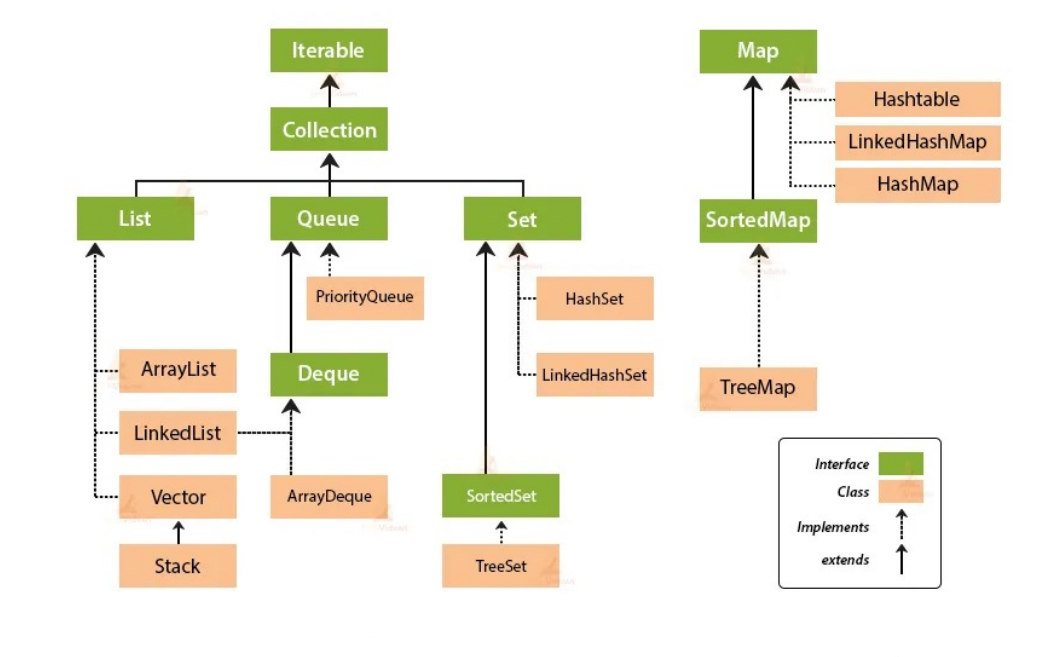
\includegraphics[scale=0.5]{img/gerarchiaJavaCollection.png}
    \caption{Gerarchia della JCF}
\end{figure}

Notiamo che i nodi rappresentati in verde rappresentano interfacce, mentre quelle in arancione sono classi. Dunque i nodi arancioni (classi) implementano specifiche interfacce che forniranno correttezza statica

Senza questo framework, le uniche strutture dati disponibili sarebbero state $Vector$ ed $Array$.

\paragraph{Iterator} Notiamo che il padre di tutti i nodi della foresta sinistra delle JFC è l'interfaccia iteratore. Questo ci permette di iterare sugli elementi delle collezioni grazie ad un generatore che restituisce un iteratore.

Un generatore solitamente è rappresentato da una funzione che restituisce un iteratore che fornisce specifici metodi per iterare sulla collezione come $itr.hasNext()$ oppure $itr.next()$. Questo ci permette di creare \textbf{astrazione} anche sul concetto di iterazioni su collezioni. Sappiamo bene che iterare su elementi di collezioni è una procedura molto ricorrente, grazie a questo espediente riusciamo a categorizzare quindi quel tipo di operazioni ricorrenti.

Bisogna avere però l'accortezza di non iterare da due diversi iteratori

sulla stessa collezione. Questo infatti porterebbe ad una situazione di inconsistenza, infatti se un iteratore apportasse una modifica alla collezione, tutti gli altri iteratori verrebbero invalidati.

\newpage

\paragraph{Astrazione e For Each} Grazie all'utilizzo dell'iteratore possiamo utilizzare nuovi

costrutti più ad alto livello, permettendoci di iterare direttamente sugli elementi di una collezione senza l'utilizzo di effettivi indici, grazie al comando $for (tipo_{elem} \: elem \: : \: collezione) $, che corrisponde al $(for \: \: \: of)$ in JS.

\subsubsection{Ereditarietà Multipla e Mixin}

Ricordiamo che Java non supporta l'Ereditarietà Multipla, ma permette ad una classe di implementare più interfacce. In generale altri linguaggi invece permettono l'Ereditarietà Multipla, ma hanno la necessità di gestire la possibilità di metodi denominati ugualmente tra classi ed anche l'occorrenza ripetuta del nodo padre della gerarchia della classe. Mostriamo un paio di esempi:

    \begin{figure}[htbp]
        \center
        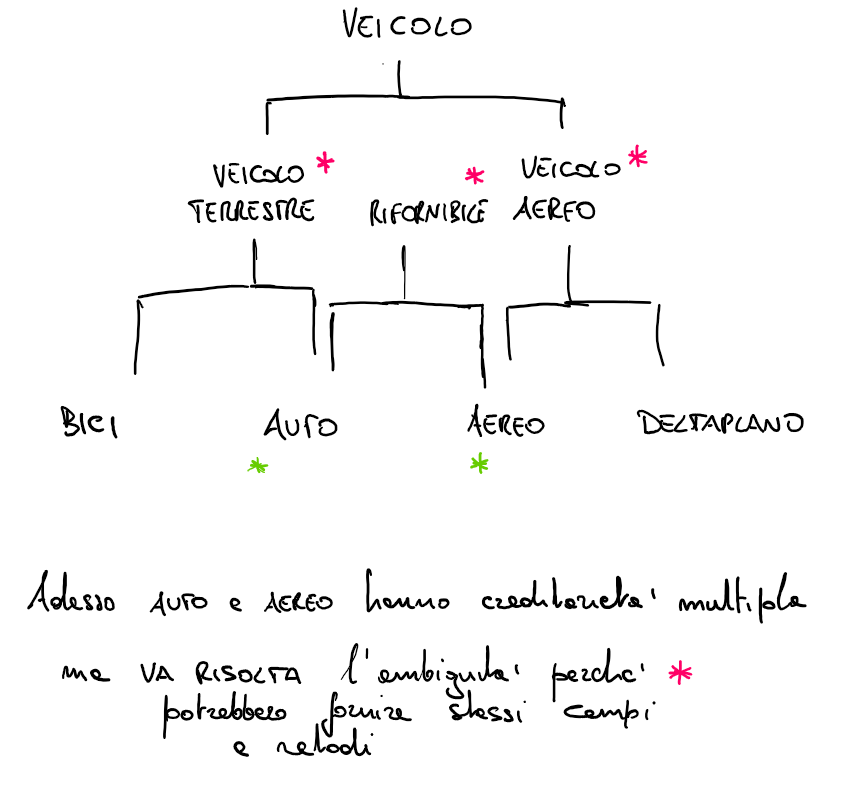
\includegraphics[scale=0.3]{img/ereditMultipla.png}
    \end{figure}

\begin{enumerate}
    \item \textbf{C++}: Permette ad una classe di ereditare da più superclassi ma questo genera il \textbf{diamond problem}, ossia che una potenziale radice super padre della gerarchia potrebbe occorrere più volte durante una risalita dell'albero. C++ risolve il problema permettendo la \textbf{virtualizzazione}, dunque conoscendo questa potenziale problematica, questo linguaggio lascia la possibilità allo sviluppatore di "ereditare virtualmente", ossia verranno skippate le superclassi intermedie, l'ipotetico metodo trovato nel padre viene puntato dalla sottoclasse stessa, skippando consapevolmente le superclassi a metà risalita.
    \begin{figure}[htbp]
        \center
        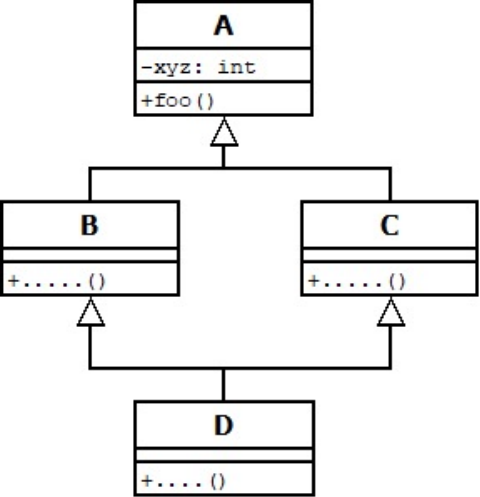
\includegraphics[scale=0.3]{img/virtualizzazione.png}
    \end{figure}
    \item \textbf{Java}: Permette di implementare più interfacce gestendo propriamente le \textbf{dispatch vectors}, senza superclassi.
    \item \textbf{Scala}: Introduce un metodo alternativo, ossia i \textbf{Mixin}. Questi sono un \textbf{interpretazione} più \textbf{dinamica} di una vera e propria \textbf{superclasse}. Una classe infatti invece di ereditare da superclassi, si definisce come rimescolamente di altre classi, il mixin infatti può essere rimescolato esso stesso ad una classe.
    
    \begin{figure}[htbp]
        \center
        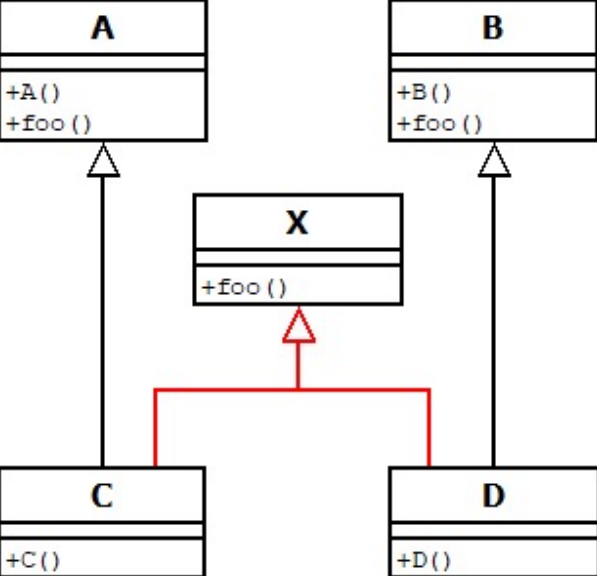
\includegraphics[scale=0.28]{img/mixin.png}
        \caption{$X$ è un mixin}
    \end{figure}

    \item \textbf{Python}: Questo linguaggio utilizza invece un altro approccio, cerca infatti di linearizzare la gerarchia delle classi per risolvere l'ambiguita sulla ricorrenza di metodi in classi diverse. Questo avviene grazie ad una sorta di buona enumerazione di tutto l'albero gerarchico, linearizzato da un algoritmo specifico, detto \textbf{Method Resolutin Order (MRO)}.

    \begin{figure}[htbp]
        \center
        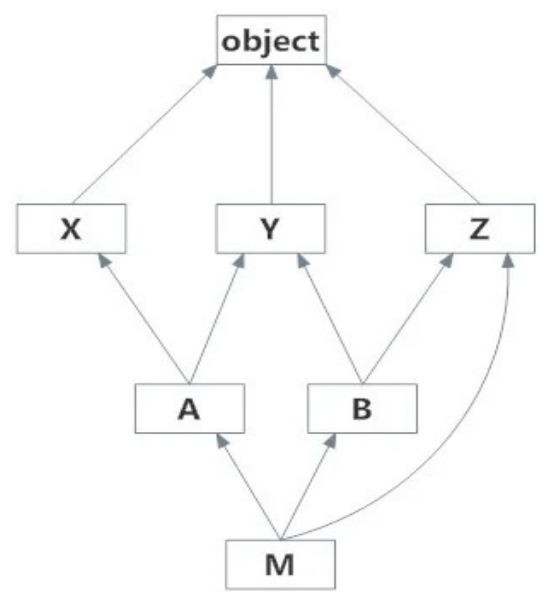
\includegraphics[scale=0.28]{img/albero_gerarchia.png}
    \end{figure}

    \begin{figure}[htbp]
        \center
        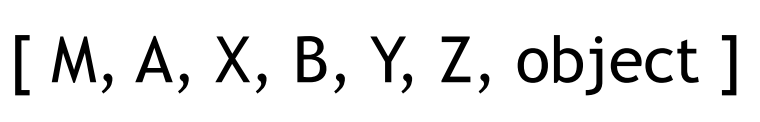
\includegraphics[scale=0.28]{img/albero_gerarchia1.png}
    \end{figure}
    
\end{enumerate}

\subsubsection{Eccezioni in Java}

Suddividiamo le eccezioni (situazioni che interrompono il flusso regolare di esecuzione) in due grandi categorie:

\begin{enumerate}
    \item \textbf{Checked}: Eccezioni che vanno dichiarate, non estendono la classe $Exception$.
    \item \textbf{Unchecked}: Eccezioni che non vanno dichiarate, ma che vengono lanciate autonomanmente quando occorre un errore a runtime. Queste estendono la classe $Exception$.
\end{enumerate}

\newpage

\subsubsection{Specifiche Metodi e Accenno Semantica Assiomatica}

Tutti i metodi sono definiti da una specifica. Questa si compone di:

\begin{enumerate}
    \item \textbf{Precondizione $\{P\}$}: Condizione iniziale su cui viene invocato il metodo. Solitamente indicato da un \textbf{REQUIRES}.
    \item \textbf{Metodo $met$}: Effettiva funzione applicata.
    \item \textbf{Postcondizione $\{Q\}$}: Condizioni richieste all'uscita dal metodo. Solitamente indicato da un \textbf{EFFECTS}.
\end{enumerate}

\vspace*{-8px}

\[ \{P\} \:\: met \:\: \{Q\} \]

Questi test permettono di ricavare errori di programmazione persino a tempo statico, fornendo più consistenza. 

\vspace*{8px}

\subsubsection{Principio di Sostituzione di Liskov}

Un oggetto di un sottotipo può sostituire un oggetto del supertipo
senza influire sul comportamento dei programmi che usano il
supertipo.

\vspace{8px}

Stabilire a tempo statico se questo principio viene rispettato è un problema indecidibile, di conseguenza si attuano delle buone pratiche ed il rispetto di determinate proprietà che mantengono il principio valido.

\vspace*{8px}

\paragraph{Proprietà da rispettare} Elenchiamo le proprietà necessarie al mantenimento di questo principio:

\begin{enumerate}
    \item \textbf{Segnatura}: E' necessario che si preservi la segnatura da supertipo a sottotipo. Se si effettua override è consentito anche ritornare un sottotipo del tipo originale.
    \vspace*{5px}
    \item \textbf{Metodi}: I metodi devono mantenere lo stesso comportamento:
    \begin{enumerate}
        \item Posso allargare le \textbf{precondizioni}.
        \item Posso restringere le \textbf{postcondizioni}.
    \end{enumerate}
    \vspace*{5px}
    \item \textbf{Proprietà}: Se la superclasse ha delle proprietà, queste devono essere mantenute nella sottoclasse. Nelle slide si mostrava un esempio su una superclasse $IntSet$ con proprietà $\{ \text{invarianza},\: \text{evoluzione} \}$, dunque anche le sottoclassi dovranno rispettare queste proprietà.

    Implicitamente vogliamo che sia sempre rispettato anche l'\textbf{incapsulamento}, senza mai permettere l'accesso non permesso a campi privati di una classe.
\end{enumerate}

\newpage

\subsection{Garbage Collection}

Dopo aver visto tutti i nuovi livelli di astrazione, possiamo immaginare di volerlo fare anche con la gestione della memoria, dato che la sua gestione manuale viola il concetto base di astrazione della programmazione.

\vspace*{8px}

\paragraph{Problematiche Gestione Manuale Memoria} Il linguaggi come il C, che lascia la gestione della memoria completamente in mano al programmatore, sono noti due problemi frequenti:

\vspace*{8px}

\begin{enumerate}
    \item \textbf{Dangling Pointers}: Dati due puntatori $ptr_{1}$ e $ptr_{2}$, uno alias dell'altro (puntano alla stessa zona di memoria), se effettuassi una $free(ptr_{1})$ allora $ptr_{2}$ punterebbe ad una zona non accessibile della memoria a causa dell'aliasing iniziale.
    \item \textbf{Memory Leak}: Perdere un riferimento ad una zona di memoria prima di deallocarla. Questo genera $garbage$, ossia memoria non riutilizzabile fino a chiusura del programma.
\end{enumerate}

\vspace*{8px}

\paragraph{Modello Memoria} Analizziamo la composizione della memoria:

\begin{enumerate}
    \item \textbf{Static}: Tabelle di supporto, variabili statiche...
    \item \textbf{Stack}: Parte di memoria che mantiene le variabili locali dei vari record di attivazione delle funzioni durante il loro ciclo di vita.
    \item \textbf{Heap}: Memoria detta dinamica, che necessita di essere gestita.
\end{enumerate}

\vspace*{8px}

\paragraph{Rootset} Solitamente una zona di memoria dell'heap, una volta allocata, viene puntata da delle variabili dello spazio dello stack oppure static. Questa variabile è definita \textbf{rootset}.

\vspace*{8px}

\paragraph{Tipi di Heap, Frammentazione e Tipi di Fit}

Un heap può essere \textbf{statico} nelle dimensioni oppure \textbf{dinamico} se ha la possibilità di ridimensionarsi. Entrambe le tipologie utilizzano una \textbf{lista libera} di supporto per tenere traccia delle locazioni occupate e quelle piene.


Un ulteriore problema da gestire nell'heap è la \textbf{frammentazione}, ossia spazio utilizzabile suddiviso in tante piccole sezioni. Elenchiamone le varie tipologie:

\begin{enumerate}
    \item \textbf{Interna}: Durante il "deposito" di una $x$ in memoria, occupo uno spazio $y$, anche se $dim_{x} << y$.
    \item \textbf{Esterna}: Tante frazioni di memoria libera ben distribuita tra blocchi di memoria occupata. Sarebbe necessario uno "shift" di fix per ricavare memoria libera unitaria.
\end{enumerate}

\newpage

\subsubsection{Metodi di Raggiungibilità}

Elenchiamo tutti i metodi di verifica di raggiungibilità, analizzandone le caratteristiche.

\vspace*{10px}

\begin{enumerate}
    \item \textbf{Reference Counting}: Mano mano tengo traccia sulla memoria heap quanti puntatori stanno facendo riferimento a quella zona. Questo funzione, ma solo per il "primo layer" di memoria puntata. Questo infatti funzionerà sui primi riferimenti da rootset ad heap, ma in caso di \textbf{puntatori circolari} nell'heap, questi non verranno trovati, causando \textbf{memory leak}.
    \vspace*{10px}
    \item \textbf{Tracing}: Verifico la raggiungibilità effettuando letteralmente una visita partendo dalla rootset. Le operazioni eseguite dopo la visita stabiliscono delle sottocategorie:
    \begin{enumerate}
        \item \textbf{Mark \& Sweep}: Durante la visita marco su $1$ bit tutti i raggiungibili, dunque il resto sarà irragiungibile. Questo mi permette di stabilire che periodicamente dovrò mettere in pausa tutto ed effettuare una pulizia dei non raggiungibili, causando uno "stop the world" event.
        Questa metodologia ha pro e contro, infatti risolve il memory leak dei riferimenti circolari, ma causa un evento di stop per effettuare la pulizia.
        \item \textbf{Coping Collection}: Descriviamo l'algoritmo di Cheney che caratterizza questa metodologia:
        \begin{enumerate}
            \vspace*{8px}
            \item \textbf{Divisione Heap}: Ho due sezioni di heap, "from-space" e "to-space".
            \vspace*{8px}
            \item \textbf{Allocazione}: Uso soltanto la parte "from-space" per allocare nuova memoria.
            \vspace*{8px}
            \item \textbf{Attivazione GC}: Le celle attive vengono copiate da "from-space" in "to-space".
            \vspace*{8px}
            \item \textbf{Inverto le parti}: Rendo la "to-space" attiva e la "from-space" disattivata.
            \vspace*{8px}
            \item \textbf{Lista Libera}: Restituisco in una lista libera tutta la parte liberata.
        \end{enumerate}
    \end{enumerate}
    \vspace*{10px}
    \item \textbf{Generational Garbage Collector}: Gestione dell'heap in base allo scope dei riferimenti, quindi chi viene creato di recente probabilmente sarà in un blocco più interno che presto si chiuderà. Questo causa la suddivisione dell'heap in generazioni, dove quelle \textbf{young} vengono cancellate e quelle \textbf{old} mantenute.
    \vspace*{10px}
    \item \textbf{Hotspot JVM}: Java suddivide tutto l'heap in $3$ generazioni, nella prima e nella seconda applica il Copying Collection, mentre nella terza applica Mark $\&$ Sweep cercando di evitare la frammentazione.

\newpage

    \subsubsection{Piccolo confronto con Rust}

    L'approccio seguito da Rust è completamente differente, infatti non fa uso di garbage collectors ma impone delle regole sulla \textbf{ownership} di ogni oggetto sull'heap. Questo permette una gestione della memoria safe ed alternativa. Elenchiamone delle caratteristiche:

    \begin{enumerate}
        \item \textbf{Ownership}: Ogni zona di memoria ha un sono \textbf{owner} (puntatore \textbf{rootset}), durante un assegnamento di puntatori viene \textbf{scambiata} la \textbf{ownership}. Quando si esce dallo scope dell'\textbf{owner}, la memoria sull'heap viene deallocata.
        \item \textbf{Borrowing}: Esiste il \textbf{borrow} in lettura o in scrittura, dunque l'\textbf{aliasing} si crea esplicitamente nello scope dell'\textbf{owner}. L'obiettivo è quello di non far coesistere aliasing e mutation, dunque segue delle regole:
        \begin{enumerate}
            \item Il riferimento è \textbf{unico} e \textbf{mutabile}.
            \item Il riferimento \textbf{non è unico} ed è \textbf{immutabile}.
        \end{enumerate}
    \end{enumerate}
    
\end{enumerate}

\section{Concorrenza}

Il primo concetto fondamentale è capire come un calcolatore moderno riesca a darci 

l'impressione che tutti i \textbf{thread} (sottoprocessi) vengano eseguiti contemporaneamente. Per assurdo se volessimo eseguire realmente $k$ processi in parallelo, allora sarebbe necessario avere anche $k$ CPU. 


\paragraph{Sistemi Multicore} Questa tipologia di sistemi possiede effettivamente multipli \textbf{core}, ma in ogni caso i $k$ processi saranno comunque di più rispetto agli $n$ core.

\[ k >> n \]

\paragraph{Concorrenza e Interleaving} Dunque la situazione reale è descritta da un \textbf{mescolamento} di esecuzioni di \textbf{thread}. Questo fenomeno è detto \textbf{interleaving}.

\paragraph{Non determinismo e Scheduler} Non è possibile descrivere l'ordine di esecuzione di thread con un automa deterministico, perchè l'ordine verrà settato da uno \textbf{scheduler}, che ha il ruolo di non far collidere due esecuzioni di processi, gestendo l'\textbf{interleaving} sopra definito. Dobbiamo anche considerare che una CPU non esegue un intero comando ad alto livello, ma ha la necessita di dividerlo in tante \textbf{istruzioni ASM}, dunque già una sola istruzione corrisponde a tante azioni diverse eseguite dalla CPU.

\paragraph{Condivisione di memoria tra processi} Due diversi processi non condivideranno mai la stessa memoria senza un preciso protocollo di sincronizzazione. Solo successivamente definiremo il \textbf{memory sharing}, ma prima di quello specifico modello si assume che due macro processi non condividano mai memoria.

\newpage

\subsection{Shared Memory vs Message Passing}

Mostriamo le differenze tra questi due principali modelli di sincronizzazione di processi (in questo caso thread).

\begin{enumerate}
    \item \textbf{Shared Memory}: Si accede alle stesse zone di memoria, adattando il comportamento dei due thread in base al valore contenuto nella zona di memoria. Mostriamo l'esempio \textbf{produttore/consumatore}:

\vspace*{10px}
\begin{lstlisting}[language = JavaScript]
    // variabili globali (memoria condivisa)
    int x = 0;
    // THREAD 1
    producer(){
        int k = 6;
        x = fattoriale(k);
    }
    // THREAD 2
    consumer(){
        while(x==0) {sleep(10);}
        print(x);
    }
\end{lstlisting}
\vspace*{-15px}

Notiamo come il secondo thread, grazie all'approccio di \textbf{busy waiting}, sta assumendo un comportamento rispetto al valore di quella zona di memoria. Questo approccio è molto inefficiente dato che il secondo thread impegna la CPU solo per un continuo check della variabile.

\vspace*{15px}

\item \textbf{Message Passing}: Questo modello invece sincronizza le esecuzioni dei due thread inviando "messaggi di check". Mostriamo un esempio in pseudocodice:

\vspace*{10px}
\begin{lstlisting}[language = JavaScript]
    // variabili globali (memoria condivisa)
    int x = 0;
    // THREAD 1
    producer(){
        int k = 6;
        x = fattoriale(k);
        send(x);
    }
    // THREAD 2
    consumer(){
        int y = receive();
        print(y);
    }
\end{lstlisting}
\vspace*{-15px}

In questo modo il \textbf{consumer} si mette in attesa del \textbf{producer} e il $send$ permetterà lo sblocco del \textbf{consumer} con il valore atteso.

\end{enumerate}

\newpage

\subsubsection{Processi vs Thread}
Definiamo differenze tra thread e processi.

\begin{enumerate}
    \item \textbf{Processi}: Elenchiamone le caratteristiche:
        \begin{enumerate}
            \item Ogni processo ha uno \textbf{spazio di memoria indipendente}. Si garantisce maggiore sicurezza ed isolamento.
            \item I processi \textbf{comunicano} tramite \textbf{meccanismi} forniti dal \textbf{sistema operativo}.
            \item I processi sono più \textbf{"pesanti"} in termini di risorse, dato che il \textbf{sistema operativo allocherà risorse} indipendenti per questi ultimi.
            \item Supportano il reale \textbf{parallelismo}.
            \item Il \textbf{crash} di un processo non influenza l'esecuzione degli altri, grazie all'isolamento definito prima.
        \end{enumerate}
    \item \textbf{Thread}: Elenchiamone le caratteristiche:
        \begin{enumerate}
            \item Possono \textbf{condividere} tra di loro \textbf{memoria}.
            \item La \textbf{comunicazione} tra thread \textbf{avviene} proprio grazie alla \textbf{memoria} che condividono.
            \item In termini di \textbf{risorse} i \textbf{thread} sono \textbf{meno "pesanti"}.
            \item Anche i thread supportano il parallelismo spaziale su core diversi.
            \item Il \textbf{crash} di questi uno di questi può compromettere anche altri thread, dato che la memoria su cui operano è condivisa.
        \end{enumerate}
\end{enumerate}

\subsection{Mini Linguaggio Imperativo ed Estensione Concorrente}

Immaginiamo un semplice linguaggio\footnote{Acquisizioni dirette delle slide del corso di Paradigmi di Programmazione 24/25} imperativo definito dalle correnti regole su grammatica e semantica, e successivamente estendiamolo con costrutti di \textbf{concorrenza}.

\begin{figure}[htbp]
    \center
    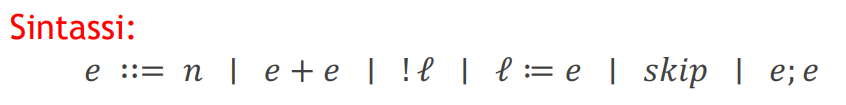
\includegraphics[scale=0.4]{img/sintassi_modello.png}
\end{figure}

\begin{figure}[htbp]
    \center
    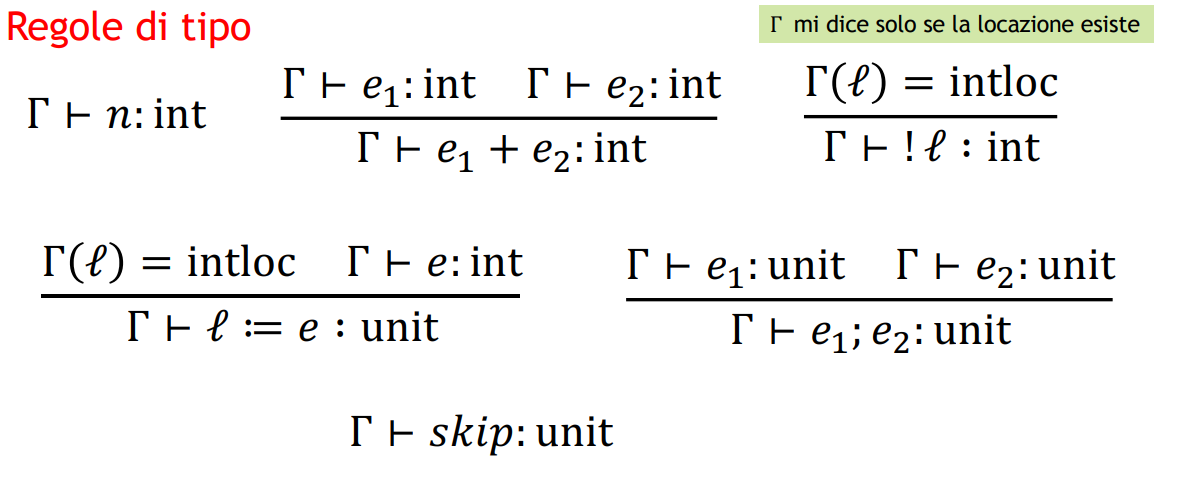
\includegraphics[scale=0.2]{img/semantica1_modello.png}
    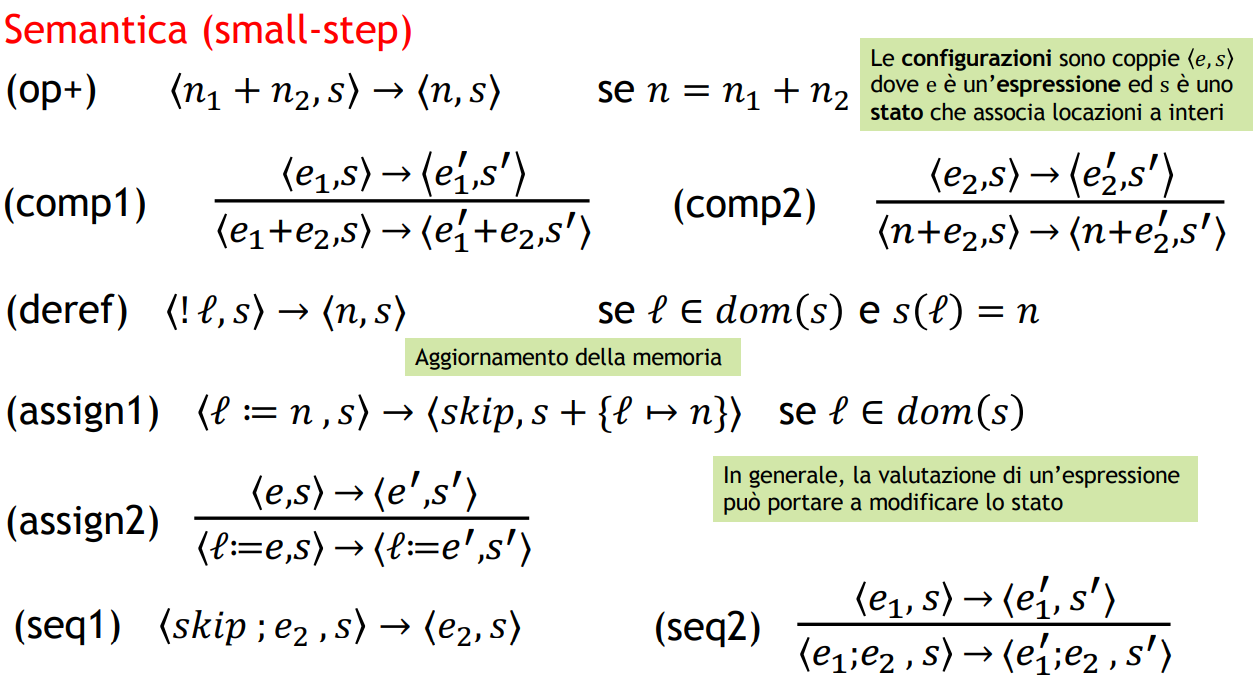
\includegraphics[scale=0.2]{img/semantica2_modello.png}
\end{figure}

\newpage

\subsubsection{Estensione Concorrente}

Aggiungiamo questi costrutti e regole d'inferenza per rendere il linguaggio capace di eseguire \textbf{composizioni di espressioni}.

\begin{figure}[htbp]
    \center
    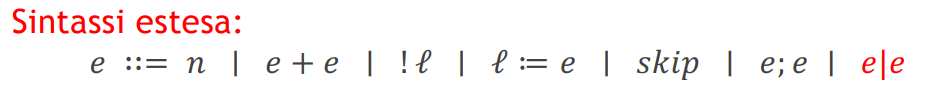
\includegraphics[scale=0.3]{img/sintassi1_modello.png}
\end{figure}

\begin{figure}[htbp]
    \center
    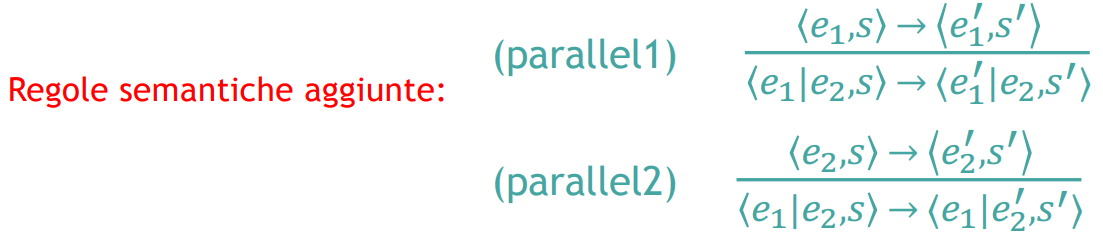
\includegraphics[scale=0.3]{img/semantica3_modello.png}
\end{figure}

Notiamo che nella grammatica abbiamo fornito \textbf{operazioni atomiche}, ossia:

\begin{enumerate}
    \item $!$ dereferenziazione
    \item $:=$ assegnamento
    \item $skip$
\end{enumerate}

\subsubsection{Lock - Meccanismo di Mutua Esclusione (Mutex)}

Forniamo a questo linguaggio un modo per poter limitare l'accesso a specifiche risorse solo ad un thread alla volta.

\paragraph{Lock/Unlock} I $lock$ sono un esempio di primitiva di sincronizzazione. Stiamo assicurando che per una determinata quantità di tempo \textbf{un solo} thread avrà accesso a specifiche risorse. Successivamente forniamo anche un \textbf{unlock} per poter sbloccare le risorse bloccate. Dunque l'accesso a delle zone di memoria richiede specifiche fasi:
\begin{enumerate}
    \item Acquisizione di un mutex (token), con il costrutto lock.
    \item Accesso esclusivo, se nessun altro thread sta già accedendo a quella memoria si può procedere con le operazioni del thread.
    \item Attesa, se un altro thread ha gìà bloccato la zona di memoria con un mutex, allora il corrente thread è messo in attesa.
    \item Rilascio, quando il thread ha finito, rilascia la memoria effettuando un unlock del rispettivo token.
\end{enumerate}

\begin{figure}[htbp]
    \center
    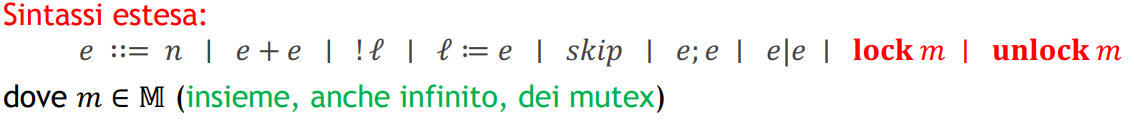
\includegraphics[scale=0.3]{img/sintassi2_modello.png}
    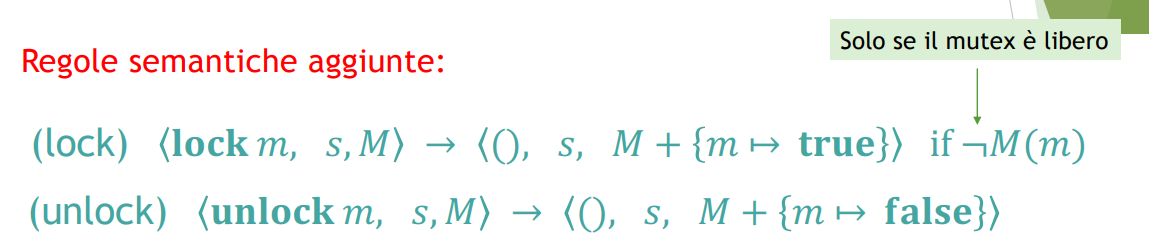
\includegraphics[scale=0.3]{img/semantica4_modello.png}
\end{figure}

\newpage

\subsection{Tipologie di Lock e Deadlocks}

L'utilizzo coerente e consistente dei lock permette una corretta gestione degli accessi concorrenti alla memoria, non permettendo a più thread di operare sulla stessa memoria contemporaneamente. Dunque ogni locazione condivisa dovrebbe essere associata ad un mutex e ogni volta che un thread inizia ad operare su quella zona di memoria dovrebbe bloccarla e rilasciarla quando ha terminato.

\subsubsection{Coarse/Fine Grained Locking}

Mostriamo due esempi "polarizzati" di utilizzo di lock:

\begin{enumerate}
    \item \textbf{Coarse Grained}: Questa strategia utilizza un unico mutex per proteggere tutte le locazioni. Questo porta ad essere sicuri di non causare mai un \textbf{deadlock}, ma \textbf{riduce} il \textbf{livello} di \textbf{concorrenza} generabile.
    \item \textbf{Fine Grained}: Questa strategia utilizza un mutex per ogni locazione bloccata dai thread. In questo modo il \textbf{livello} di \textbf{concorrenza} generabile è \textbf{alto} ma si può andare in contro a \textbf{deadlock}.
\end{enumerate}

\subsubsection{Deadlocks e Risoluzione}

Un \textbf{deadlock} è una situazione nella quale l'utilizzo improprio dei lock causa un blocco dell'intero programma. L'esempio classico è quello dell'\textbf{attesa circolare}. 

\vspace*{-30px}

\begin{multline}
    \\ \text{(ATTESA CIRCOLARE)} \\Thread_{1} \:\: blocca \:\: Risorsa_{1} \:\: ed \:\: attende \:\: Risorsa_{2} \\ mentre \\ Thread_{2} \:\: blocca \:\: Risorsa_{2} \:\: ed \:\: attende \:\: Risorsa_{1} \\
\end{multline}

Questa è una delle cause di blocco dei programmi che vanno killati.
Esistono però metodologie per prevenire, evitare o risolvere queste occorrenze del deadlock:

\begin{enumerate}
    \item \textbf{Deadlock Prevention}: Si stabiliscono precise regole \textbf{statiche} tali per cui non possono verificarsi deadlock. Mostriamo esempio di regola:
    \begin{enumerate}
        \item \textbf{2-Phase Locking}: Si stabilisce un ordine su tutti i mutex, dunque ogni thread dovrà:
        \begin{enumerate}
            \item Eseguire dei lock in ordine \textbf{crescente}.
            \item Dopo aver operato sulla memoria, esegue degli unlock in ordine \textbf{decrescente}.
        \end{enumerate}
    \end{enumerate}
    \item \textbf{Deadlock Avoidance}: Si effettuano controlli a \textbf{runtime} che permettono di stabilire se si sta per causare un deadlock e si evita di incorrere in quella situazione.
    \item \textbf{Deadlock Recovery}: Si permette al programma di cadere in un deadlock, ma se ciò accade a \textbf{runtime} si ripristina uno stato senza deadlock. 
\end{enumerate}

\newpage

\subsection{Concorrenza nei Linguaggi Moderni}

Analizziamo dei tipi di concorrenza in linguaggi moderni.

\subsubsection{Java e Multithreading}

Java offre la classe $Thread$ che permette la gestione della concorrenza. Mostriamo un esempio:

\vspace*{10px}
\begin{lstlisting}[language = JavaScript]
    class Main {
        public static void main(String[] args) {
            Runnable r = new Runnable() {
            // Creazione classe anonima
            public void run() { // Sovrascrittura
                System.out.println("Hello Thread!");
                }
            };
            Thread t = new Thread(r);
            // Creazione del thread
            t.start(); // Avvio del thread
        }
    }
\end{lstlisting}
\vspace*{-15px}

Dunque questo schema fornisce uno stack per ogni oggetto $Thread$, ma la gestione dell'Heap è in $Shared \: Memory$.

\paragraph{Locking in Java} Anche il Java permette di il lock di risorse utilizzate da un thread.

\begin{enumerate}
    \item \textbf{Synchronized [Metodo] - Coarse Grained}: Il costrutto \textbf{synchronized} permette di lockare le risorse utilizzate da un thread. Dunque verranno bloccate tutte le risorse utilizzate fino alla conclusione di un determinato metodo.
    \item \textbf{Synchronized [Blocco] - Fine Grained}: Quando non vogliamo bloccare tutte le risorse di un metodo possiamo utilizzare il $synchronized$ di blocco, ridimensionando la portata del lock. Questo utilizzo può causare deadlocks.
\end{enumerate}

\subsubsection{Esempi in altri linguaggi}

\begin{enumerate}
    \item \textbf{JavaScript}: Offre $callback$, $Promise$, $async/await$ che regolano la sincronizzazione in maniera "funzionale".
    \item \textbf{Go/Erlang}: Permettono la sincronizzazione (message passing) tramite canali di comunicazione.
    \item \textbf{Kotlin}: Gestisce la concorrenza tramite un albero di gerarchia delle attività.
    \item \textbf{Haskell}: Gestisce le transazioni di database, ossia operazioni atomiche eseguite su memoria condivisa: in caso di conflitto vengono annullate e ripetute.
\end{enumerate}

\newpage

\end{document}